Before the agents described in the Chapter 2 will be implemented, we will first implement a new BSE system that can handle more complex order types and adapt the time system. This chapter will consists of Base Line results, both taken from previous literature and from running in the original BSE. These Base Line results will then be used to compare the results from running each agent (ZIP, ZIC and Sniper) in the new system. If the behaviour is similar, then we can conclude that the system has been implemented correctly. However, as the system is developed, some parameters of the agents may have to be adapted, but the overall behaviour will be the same. 

\section{Base Line Results} 
Base Line results act as a standard which can be expected from the agents by running in a homogeneous market. These results are the indicator, apart from the unit and integration testing, that ensures the market is stabilized and performs as expected. The following graphs will illustrate the transaction prices in each homogeneous market. The following results are from running in the original BSE with equilibrium price of 100 in a homogeneous market with 31 agents on each side of the book. The period length 180 is chosen to match those in previous literature in order to compare the results of the current implementation and previous established results. 

In addition, the experiments will compare \textbf{Smith's alpha} which is the standard deviation of the transaction price around the equilibrium. The equation is given by 

\begin{equation}
\alpha = \frac{100}{P_0}\sqrt{\sum_{t=0}^{n} \frac{(P_t - P_0)^2}{|T|} }
\end{equation}
where $P_0$ = equilibrium price 
\newline $P_t$ = price at transaction t 
\newline $T$ = number of total transactions in the run
\newline $n$ = $n_{th}$ transaction in the run

\begin{table}[h]
\centering
\begin{tabular}{ |m||p{4cm}|} 
\hline
\textbf{Base Line agents experiment}& \textbf{Smith's alpha value} \\
\hline
\hline
Kaplan's Sniper & 49.73 \\ 
\hline
ZI-C & 63.5\\ 
\hline
ZI-P & 24.8 \\ 
\hline
\end{tabular}
\caption{Smith's alpha value of each base line experiment}  
\end{table}
\FloatBarrier

The ZI-P agent has the lowest Smith's alpha value out of the three agents because it is the best at convergence to the equilibrium while the ZI-C agent has the highest value because the oscillation in its transaction prices is very high. 

\subsection{Kaplan's Sniper}
The Kaplan's Sniper is one of the agents implemented in the original version of the BSE. The sniper waits until near the end of the period, then submits or ``snipe" its order. This is consistent with Figure \ref{fig:Sniper_org_all} where the transaction only occurs near the end of the time period or when $t = 160$.

\begin{figure}[h]
  \begin{subfigure}[b]{0.5\textwidth}
    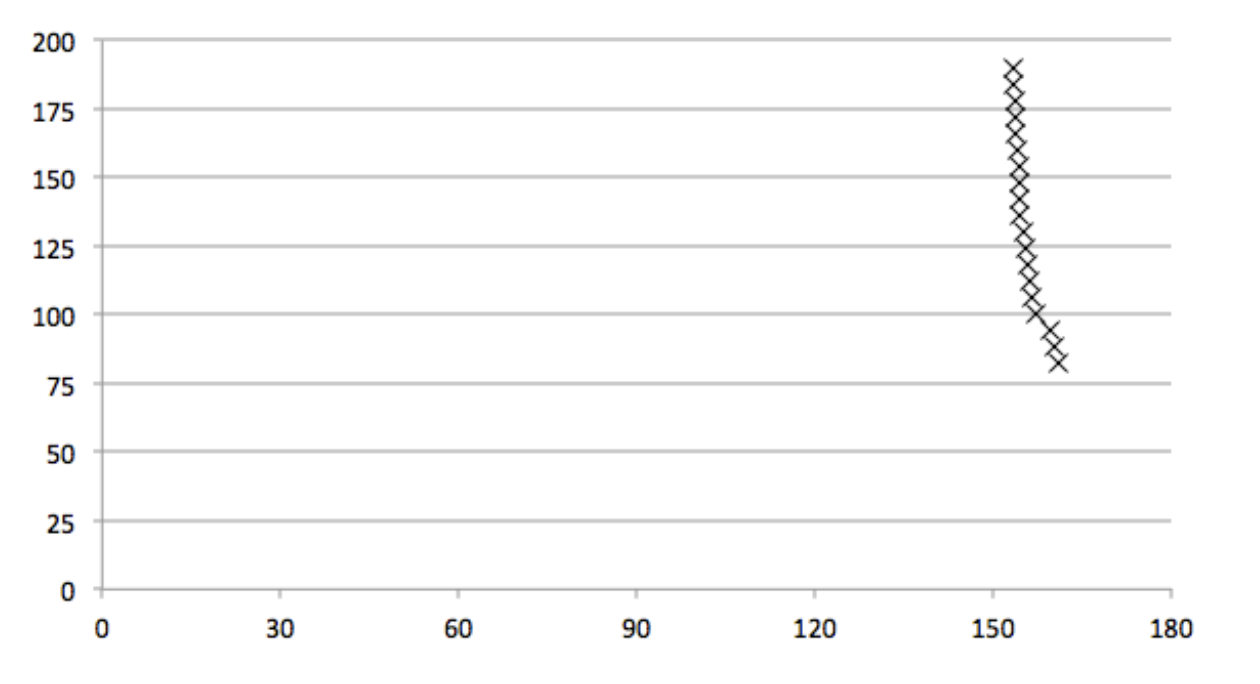
\includegraphics[width=7cm, height=7cm]{Dissertation/images/base_line/SNPR_lit.png}
    \caption{Previous Literature result \cite{BSE_lit}} 
    \label{fig:Sniper_lit}
  \end{subfigure}
  %
  \begin{subfigure}[b]{0.5\textwidth}
    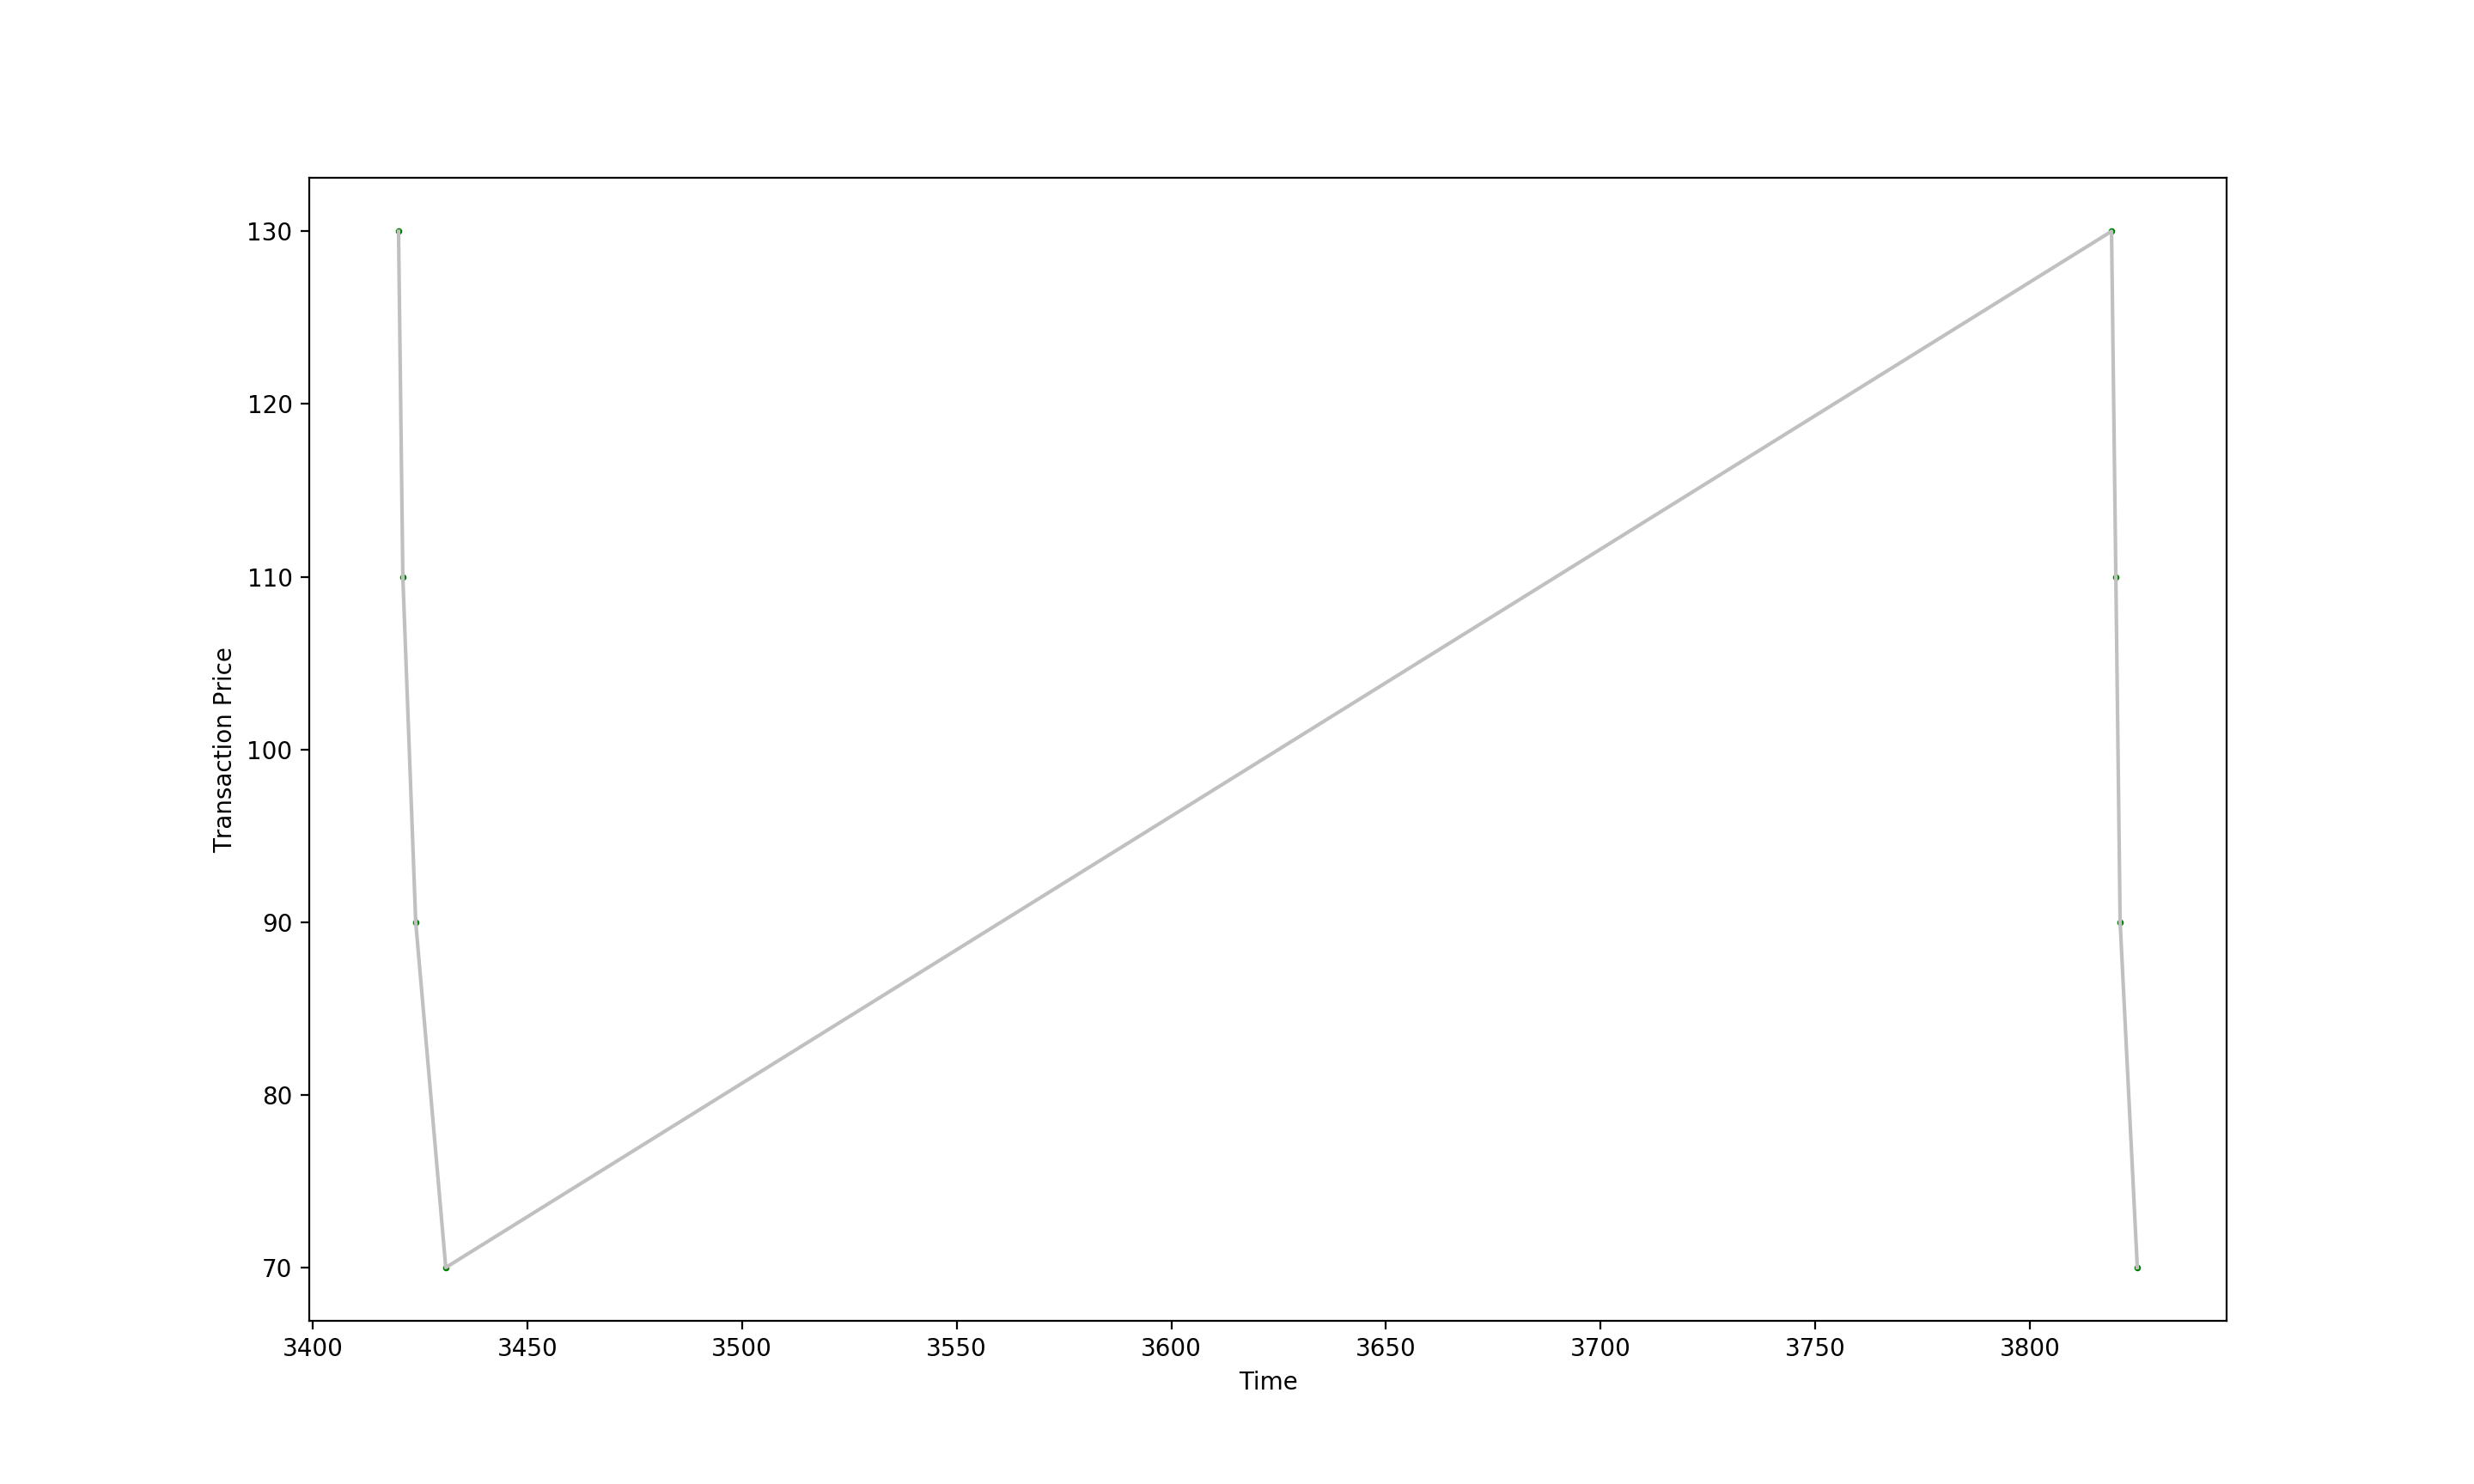
\includegraphics[width=7cm, height=7cm]{Dissertation/images/base_line/sniper.png}
    \caption{Original BSE result}
    \label{fig:Sniper_original}
  \end{subfigure}
\caption{Comparison of 62 Sniper homogeneous transaction diagram with 100 price equilibrium from previous literature and original BSE result} 
\label{fig:Sniper_org_all}
\end{figure}
\FloatBarrier

\subsection{ZI-C}
ZI-C or Zero-Intelligence Constrained is another agent implemented in the original BSE. An expected behaviour of a market consisting of only ZI-C agents is a non-convergence transaction price. This is consistent with the Figure \ref{fig:ZIC_org_all} below where at the end of the transaction period, the price does not converge to the equilibrium but instead exhibits a volatile price changes over the time period. 

\begin{figure}[h]
  \begin{subfigure}[b]{0.5\textwidth}
    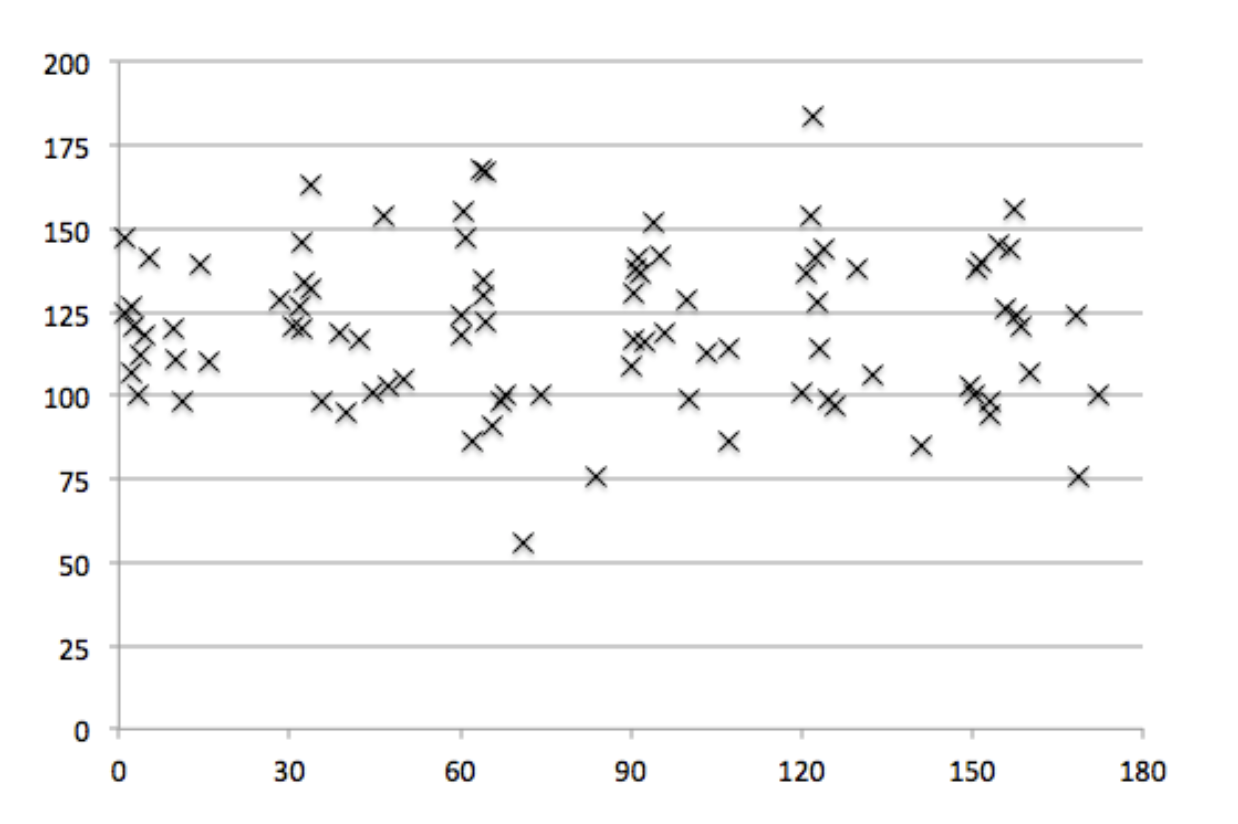
\includegraphics[width=7cm, height=7cm]{Dissertation/images/base_line/zic_lit.png}
    \caption{Previous Literature result \cite{BSE_lit}} 
    \label{fig:1}
  \end{subfigure}
  %
  \begin{subfigure}[b]{0.5\textwidth}
    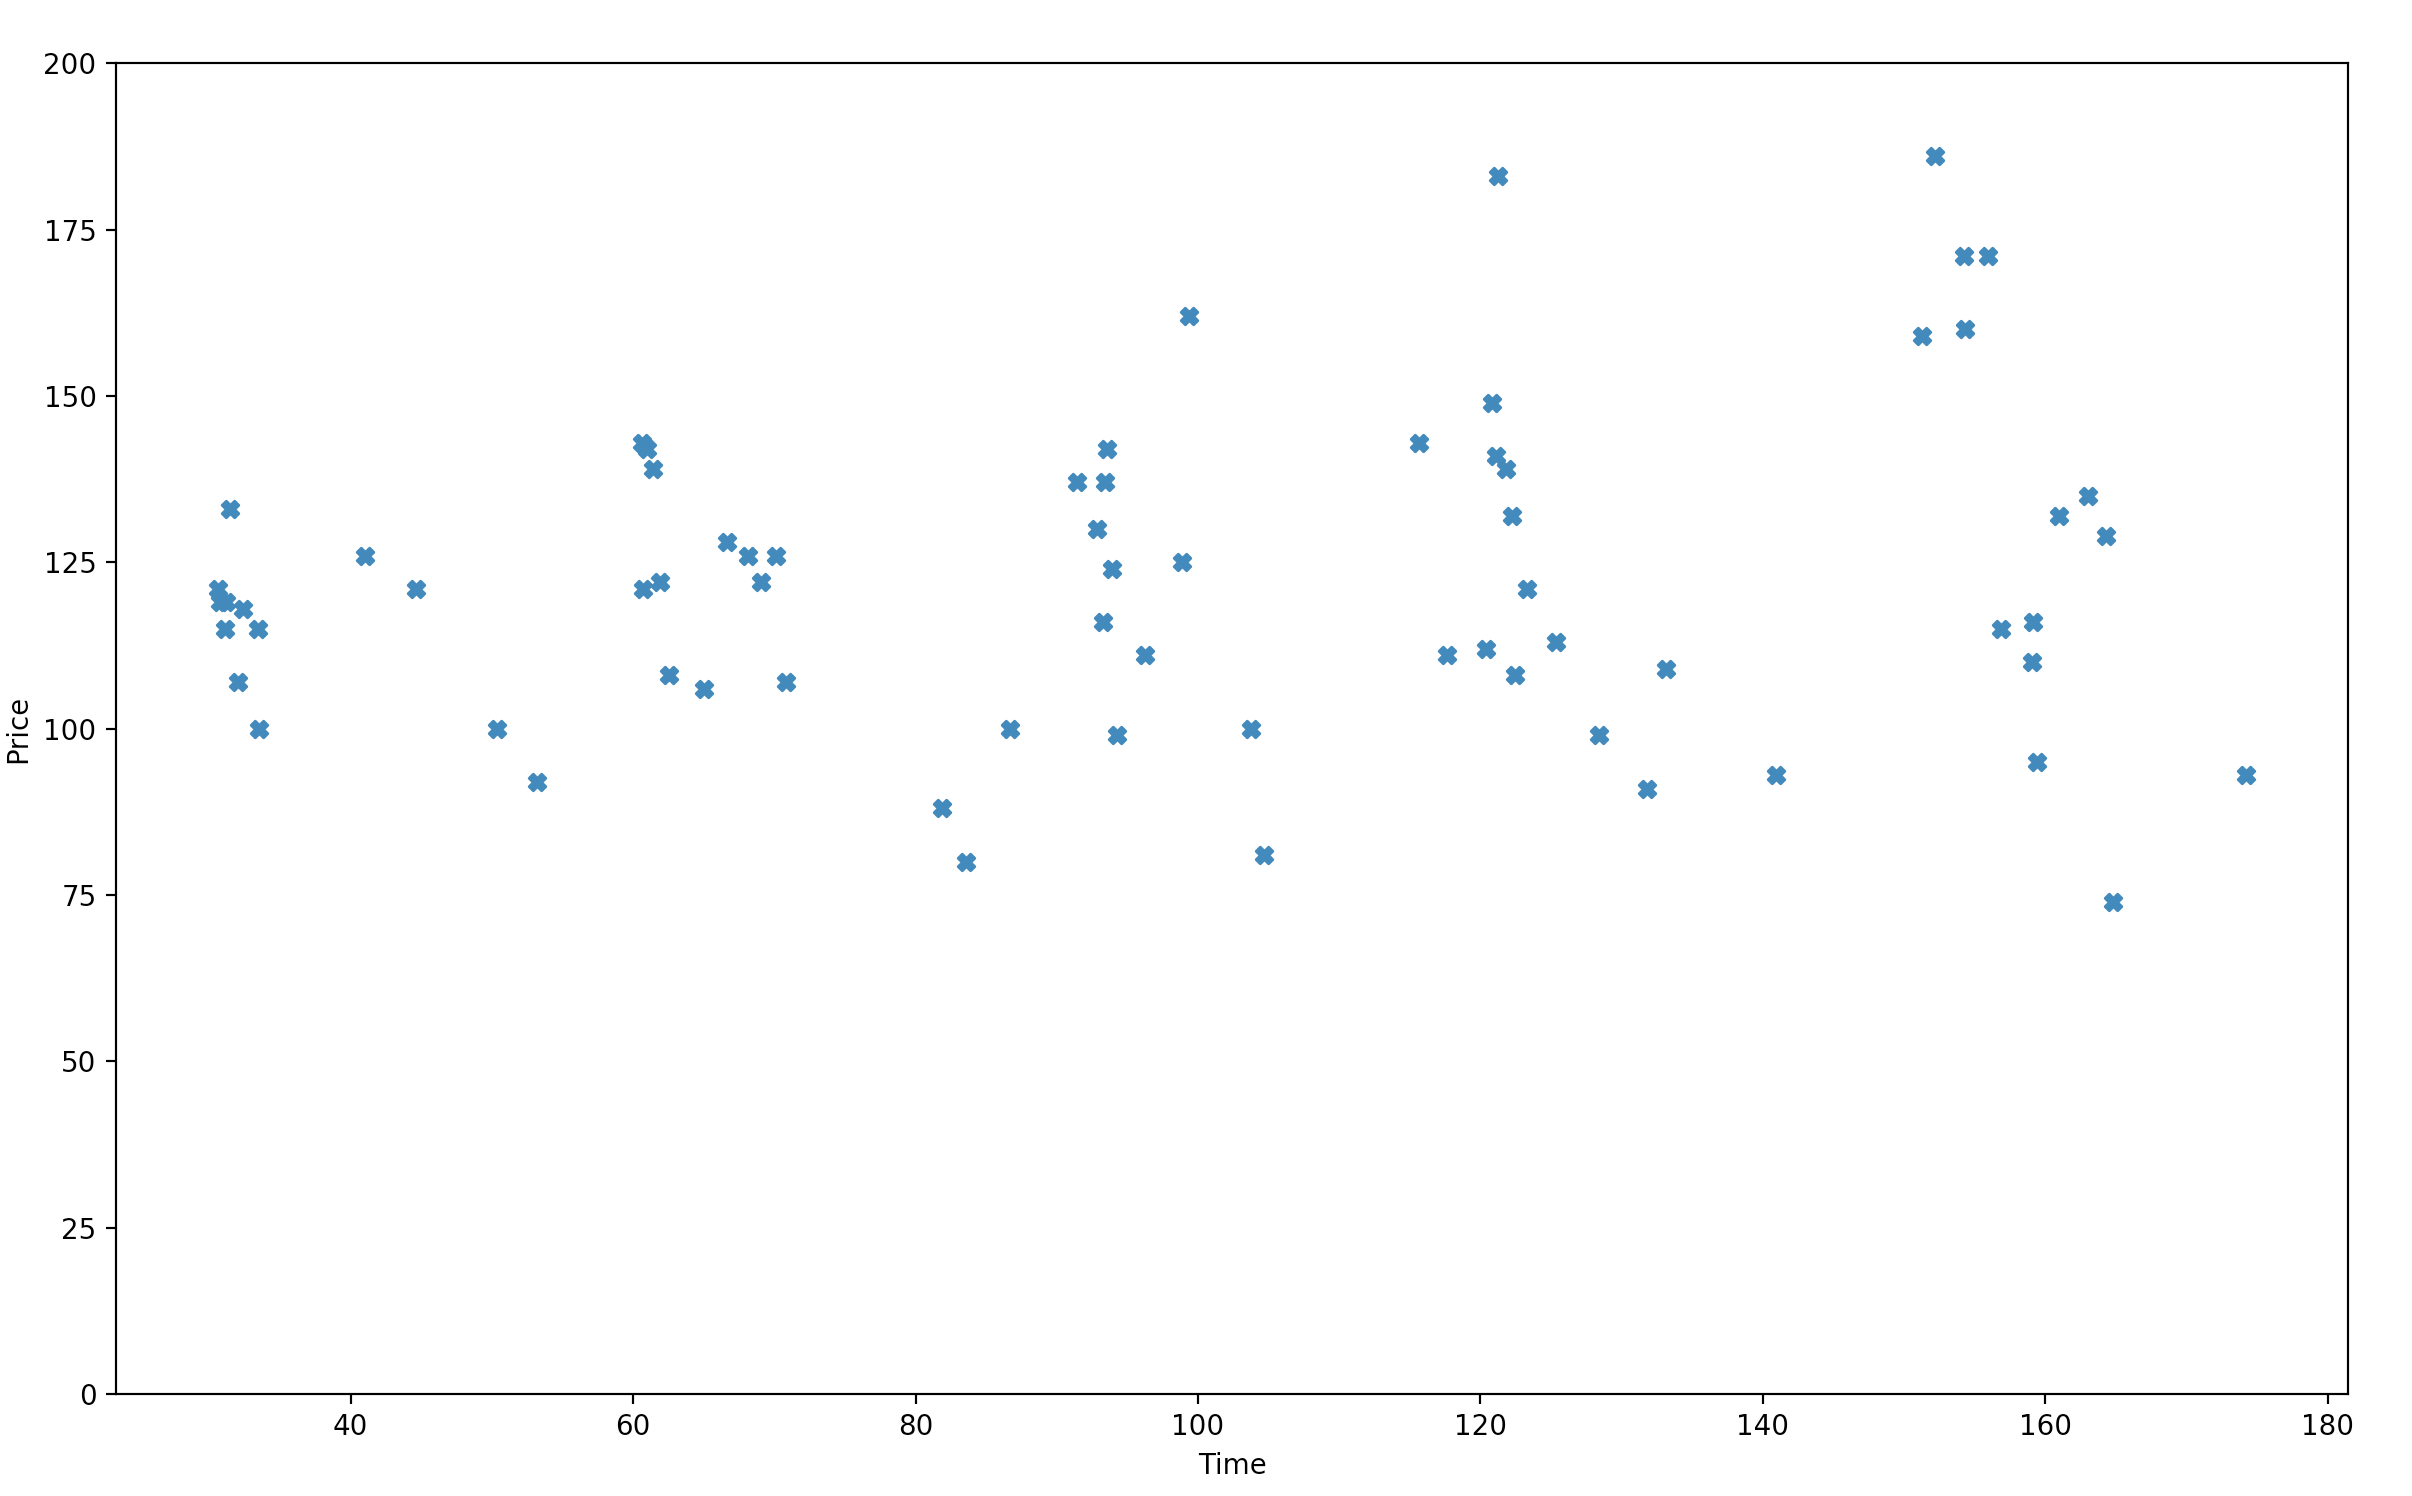
\includegraphics[width=7cm, height=7cm]{Dissertation/images/base_line/ZIC.png}
    \caption{Original BSE result}
    \label{fig:2}
  \end{subfigure}
\caption{Comparison of 62 ZI-C homogeneous transaction diagram with 100 price equilibrium from previous literature and original BSE result} 
\label{fig:ZIC_org_all}
\end{figure}
\FloatBarrier


\subsection{ZI-P}
ZI-P or Zero-Intelligence Plus is the agent that, in a homogeneous market, does produce a market where the transaction price which converges to the equilibrium. A market of ZI-P agents is a good indicator to test the market structure and functions. In the Figure \ref{fig:ZIP_org_all} below, the transaction price first fluctuates early in the transaction period but then converges towards 100 in the end of the session.  

\begin{figure}[h]
  \begin{subfigure}[b]{0.5\textwidth}
    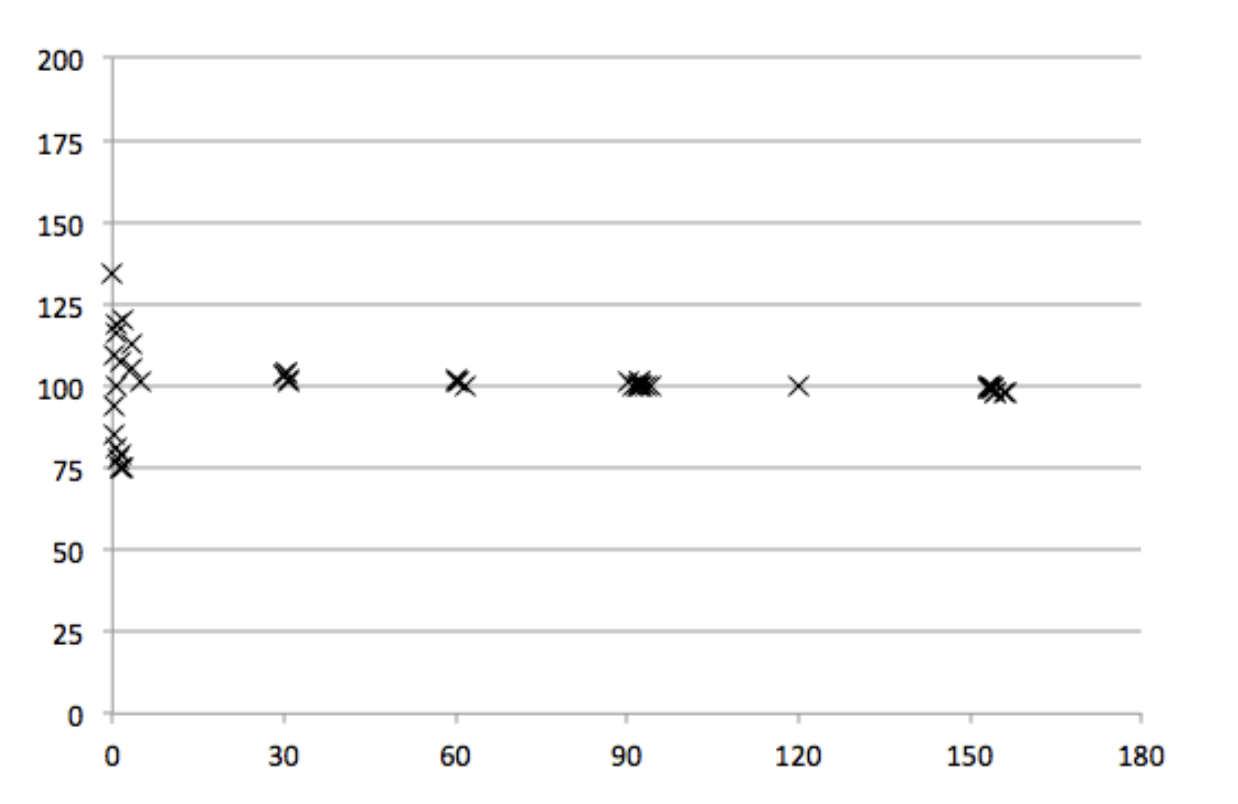
\includegraphics[width=7cm, height=7cm]{Dissertation/images/base_line/zip_lit.png}
    \caption{Previous Literature result \cite{BSE_lit}} 
    \label{fig:1}
  \end{subfigure}
  %
  \begin{subfigure}[b]{0.5\textwidth}
    \includegraphics[width=7cm, height=7cm]{Dissertation/images/base_line/zip.png}
    \caption{Original BSE result}
    \label{fig:2}
  \end{subfigure}
\caption{Comparison of 62 ZI-P homogeneous transaction diagram with 100 price equilibrium from previous literature and original BSE result} 
\label{fig:ZIP_org_all}
\end{figure}
\FloatBarrier


\section{Results after implementing complex order types} 
These results are from tests ran with the same configuration as the Base Line tests in section 3.1. These tests are ran after the LOB has been re-configured to be able to accept more than one type of order (Market Order as well as Limit Order) in addition to more than one quantity. The tests are ran with the same time step as the original BSE. Table 3.2 illustrates the similarities between the alpha values between each 2 configurations which is the evidence that the agents are acting as expected.  

\begin{table}[h]
\centering
\begin{tabular}{ |m||p{4cm}|p{4cm}|} 
\hline
\textbf{Agents}& \textbf{Base Line Smith's alpha value}& \textbf{Complex order type Smith's alpha value} \\
\hline
\hline
Kaplan's Sniper & 49.73  & 49.51 \\ 
\hline
ZI-C  & 63.5 & 64.3\\ 
\hline
ZI-P & 24.8 & 22.4 \\ 
\hline
\end{tabular}
\caption{Smith's alpha value after implementing complex order types}  
\end{table}
\FloatBarrier


\subsection{Kaplan's Sniper}
As expected, the Sniper only submits orders near the end of the session, which makes the first transactions only appear after $t = 160$.  
\begin{figure}[h]
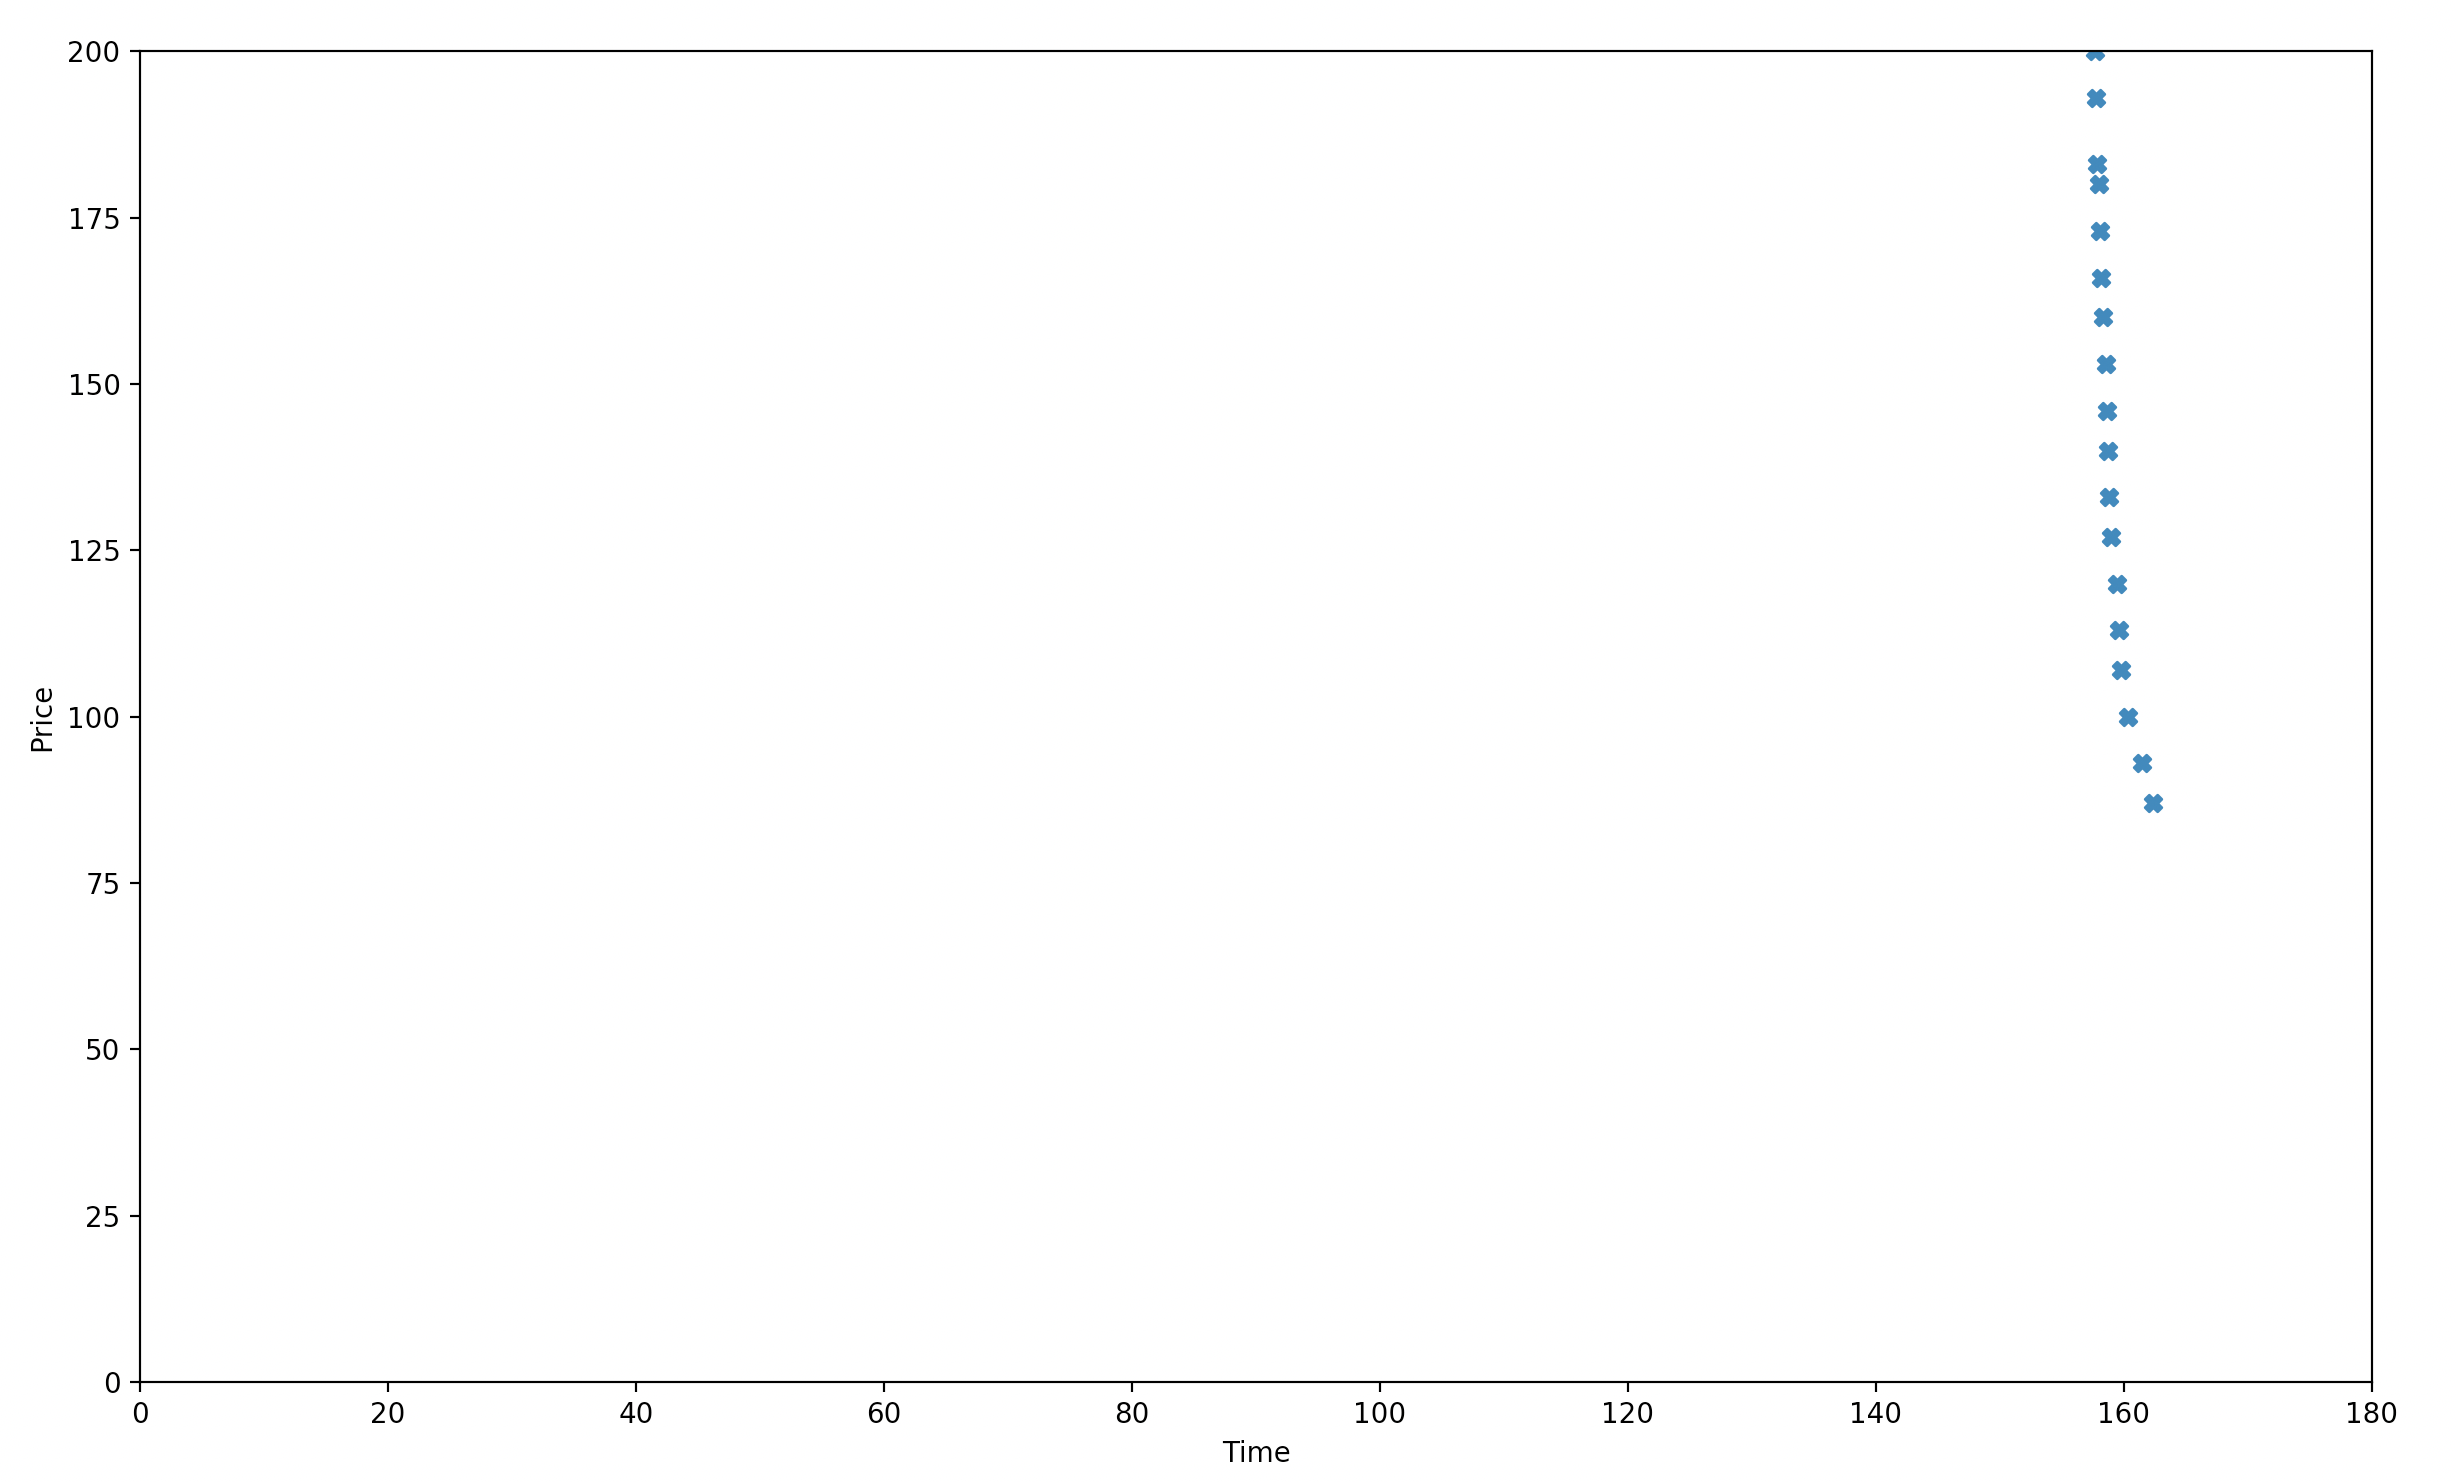
\includegraphics[ height=7cm]{Dissertation/images/change1/snpr.png}
\caption{62 Sniper agents homogeneous market transaction diagram with 100 price equilibrium from complex order types implementation} 
\end{figure} 
\FloatBarrier

\subsection{ZI-C}
ZIC's behaviour in the new LOB is still similar to the one ran in the original BSE. The transaction price does not converge in any period of the session. 

\begin{figure}[h]
\includegraphics[ height=7cm]{Dissertation/images/change1/zic.png}
\caption{62 ZI-C agents homogeneous market transaction diagram with 100 price equilibrium from complex order types implementation} 
\end{figure} 
\FloatBarrier

\subsection{ZI-P}
ZIP illustrates a convergence to the 100 equilibrium as expected. 

\begin{figure}[h]
\includegraphics[ height=7cm]{Dissertation/images/change1/zip.png}
\caption{62 ZI-P agents homogeneous market transaction diagram with 100 price equilibrium from complex order types implementation} 
\end{figure} 
\FloatBarrier

\section{Results after implementing McG action step} 
This section illustrate the results with same test configurations on the BSE with McG action step. The McG action step is similar to the BSE except that it does not divide the individual time-step by the number of buyers and sellers then select them randomly. The McG action-step loops through every trader in each step, allowing the trader to have a chance to act in all the time steps. The time period selected is 180 * 62 = 11,160 which is equivalent to the 180 time step in original BSE time-step. In addition, the interval is changed to be 10\% of the time-step for the customer order (price assignments) which is 1,860 in the McG and 30 in the original BSE. The results of the tests are illustrated below. 

\begin{table}[h]
\centering
\begin{tabular}{ |m||p{4cm}|p{4cm}|p{4cm}|} 
\hline
\textbf{Agents}& \textbf{Base Line Smith's alpha value} & \textbf{Smith's alpha value for section 3.2} & \textbf{Implemented McG action-step Smith's alpha value} \\
\hline
\hline
Kaplan's Sniper & 49.73  & 49.51 & 50.1 \\ 
\hline
ZI-C & 63.5 & 64.3 & 67.3\\ 
\hline
ZI-P & 24.8 & 22.4 & 25.4 \\ 
\hline
\end{tabular}
\caption{Smith's alpha value after implementing McG action step}  
\end{table}
\FloatBarrier

\subsection{Kaplan's Sniper}
As expected, the Sniper only submits orders near the end of the session, which makes the first transactions only appear after $t = 9000$. However, Figure \ref{fig:sniper_wrong} suggests that the behaviour of the Sniper agent is not entirely the same as there are similar transactions from the agents submitting two sets of similar orders in the end of the period. This is partly because the gap between 9,000 - 11,160 is much higher than 160 - 180 in previous experiments. Therefore, the agents have time to submit two different sets of orders. This suggests that there needs to be some adaptation to the agent's values in order to retain the behaviour it has in the Base Line experiment Figure \ref{fig:Sniper_org_all}. 

\begin{figure}[h]
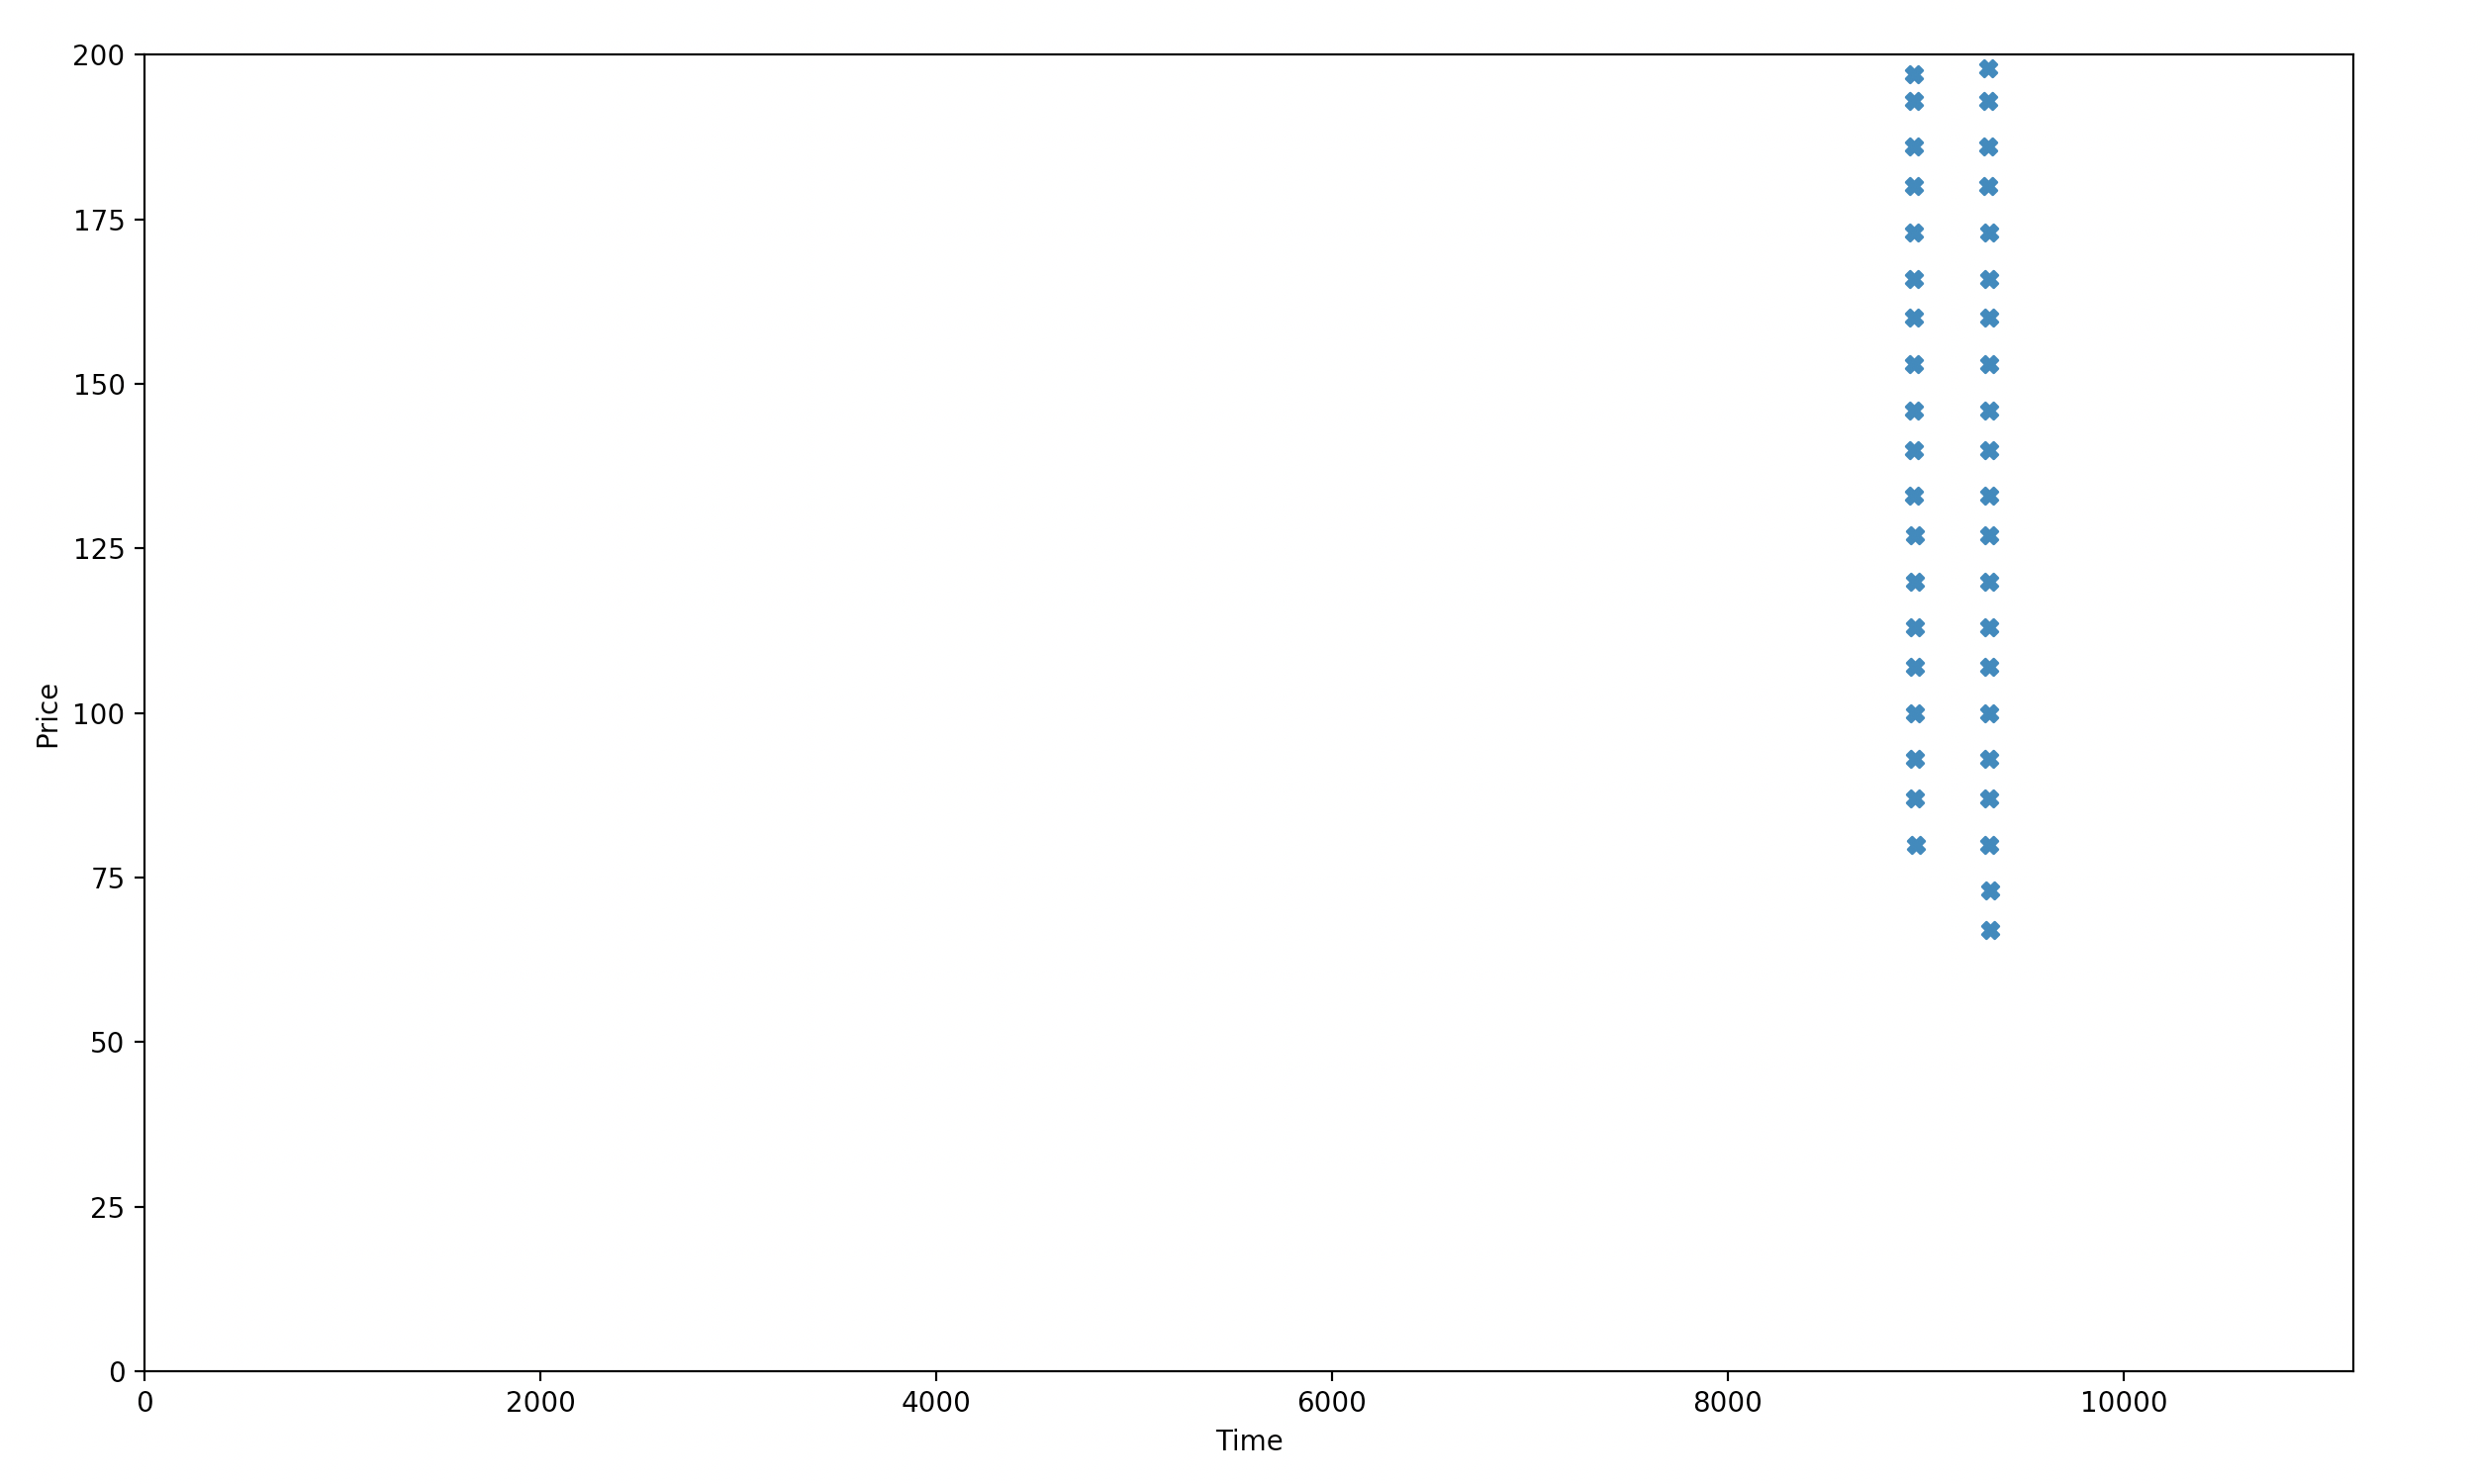
\includegraphics[ height=8cm]{Dissertation/images/snpr_adapted/2lines.png}
\caption{62 Sniper agents homogeneous market transaction diagram with 100 price equilibrium from complex order types implementation} 
\label{fig:sniper_wrong}
\end{figure} 
\FloatBarrier

After reducing the lurk threshold from 0.2 to 0.1, the agent behaviour now matches the base line results. 

\begin{figure}[h]
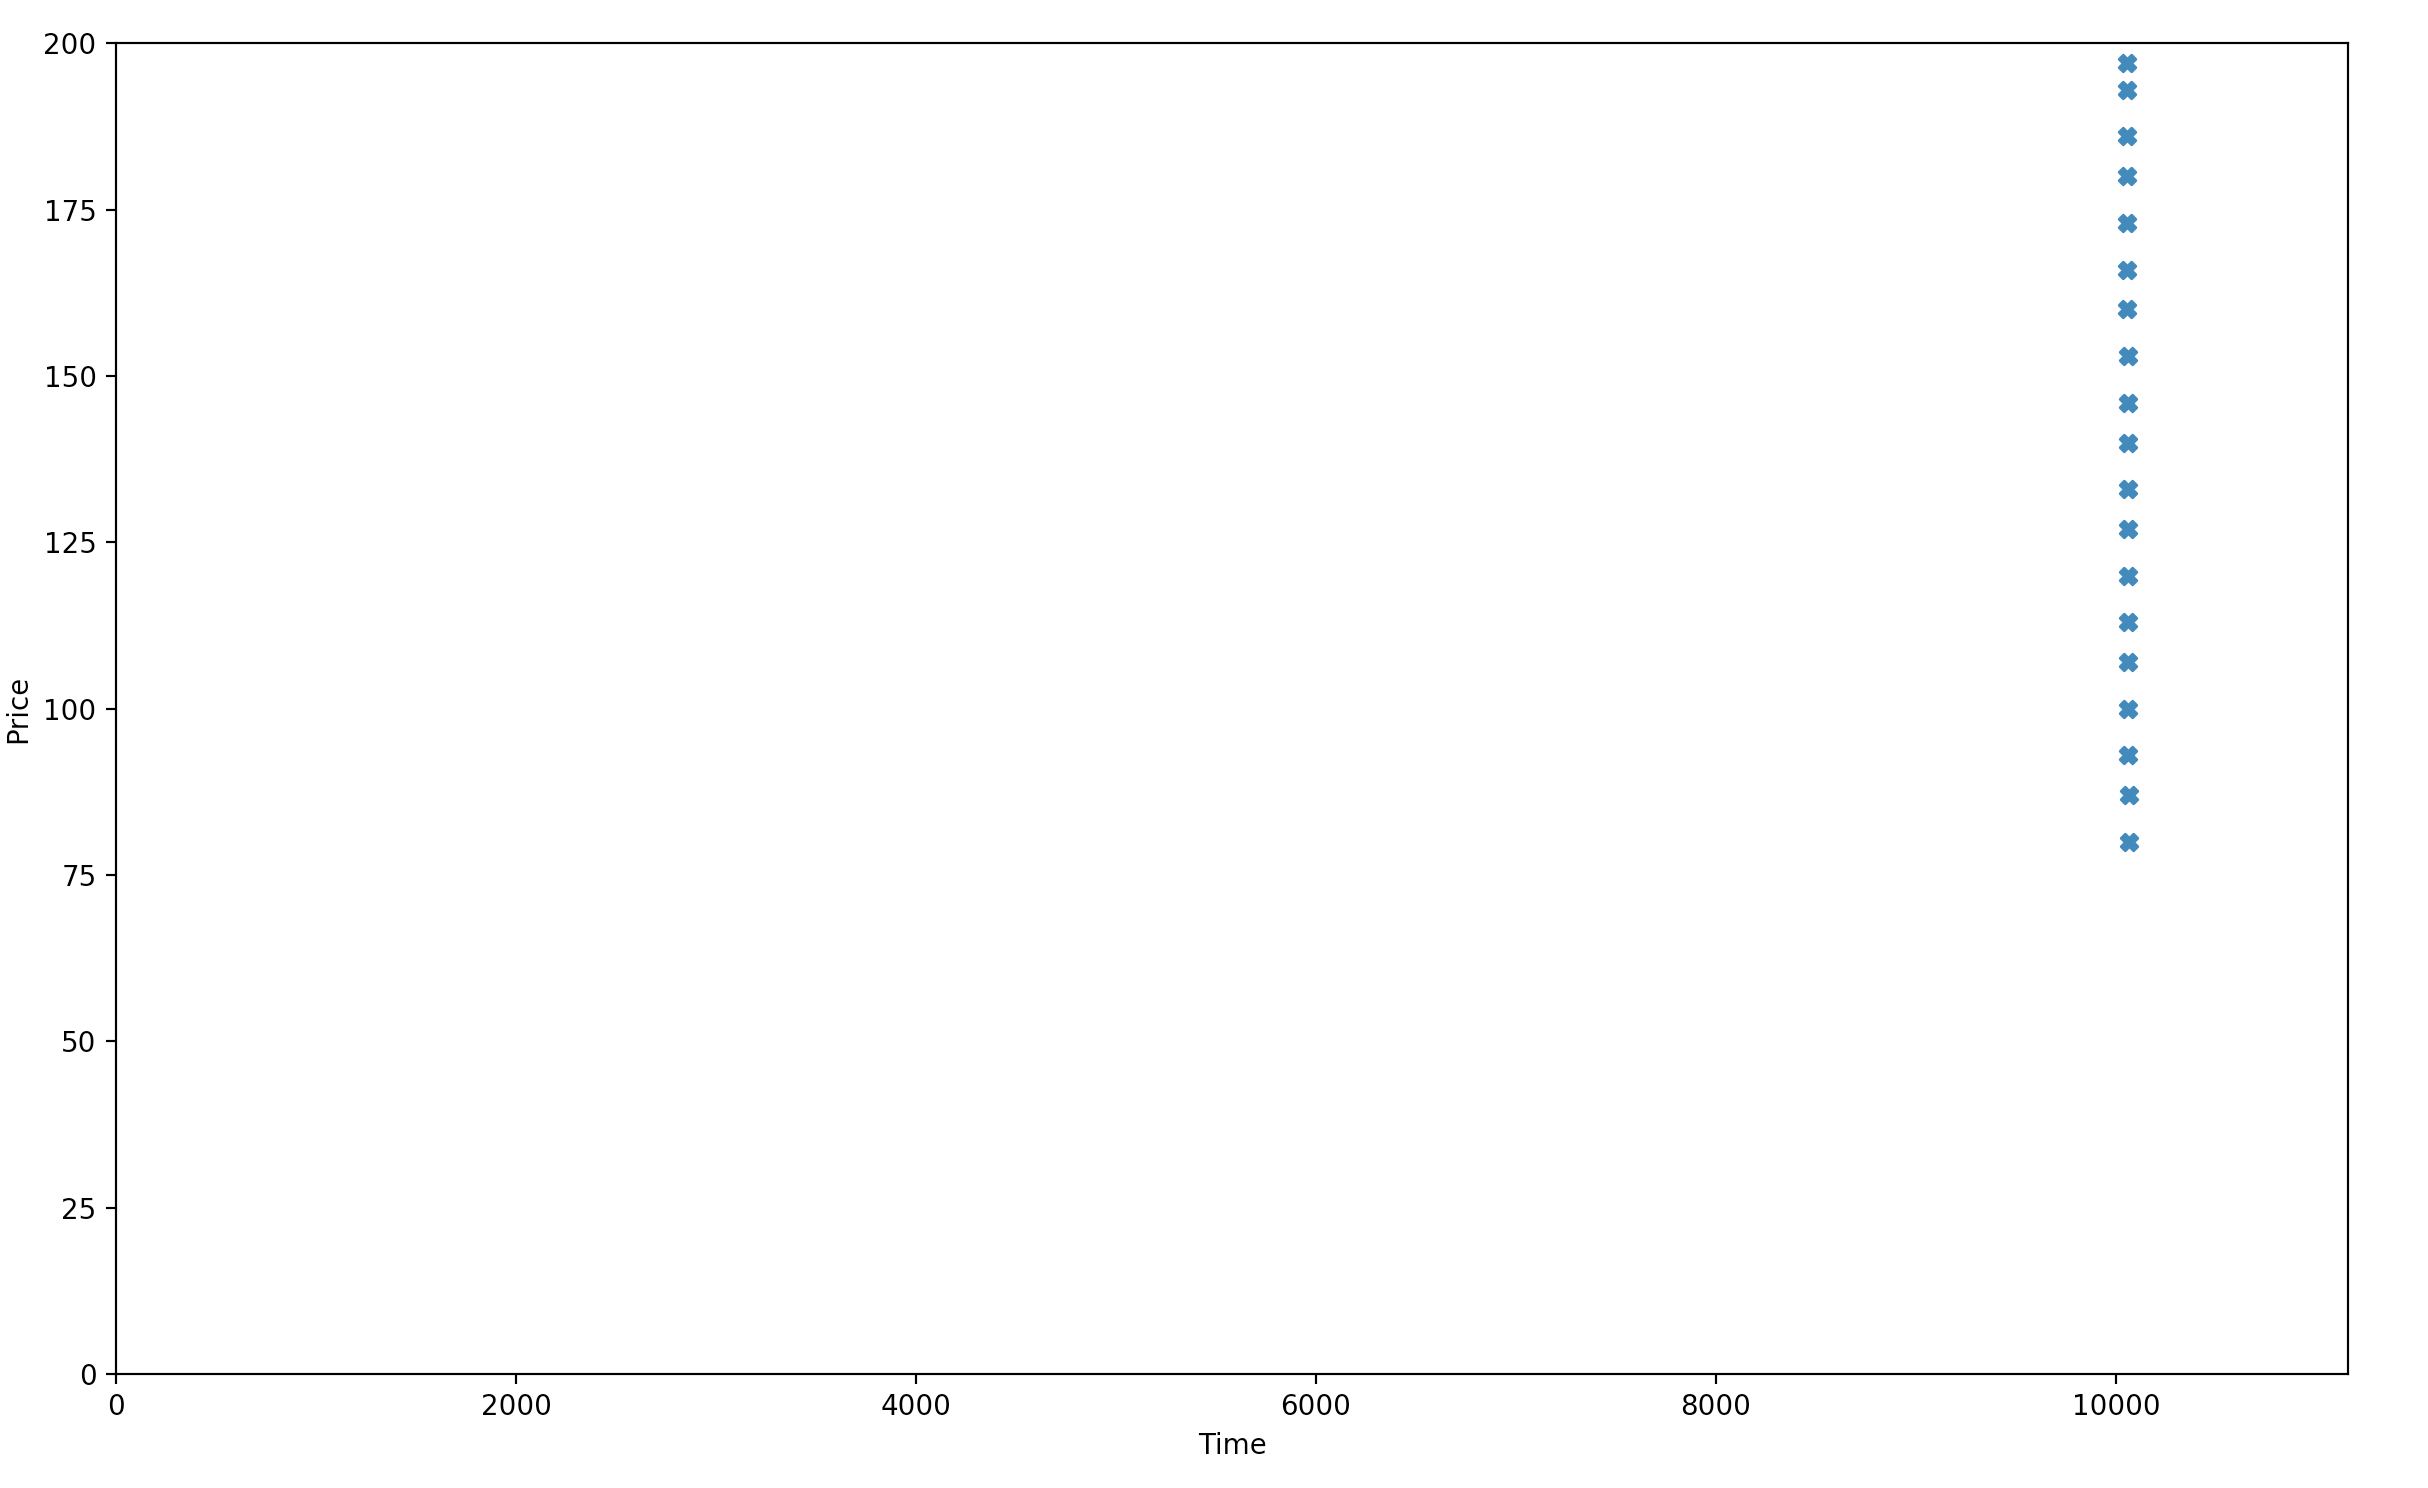
\includegraphics[ height=8cm]{Dissertation/images/snpr_adapted/adapted.png}
\caption{Adapted Sniper agent with Lurk threshold = 0.1}
\label{fig:SNIPER_FINAL}
\end{figure} 
\FloatBarrier

\begin{figure}[h]
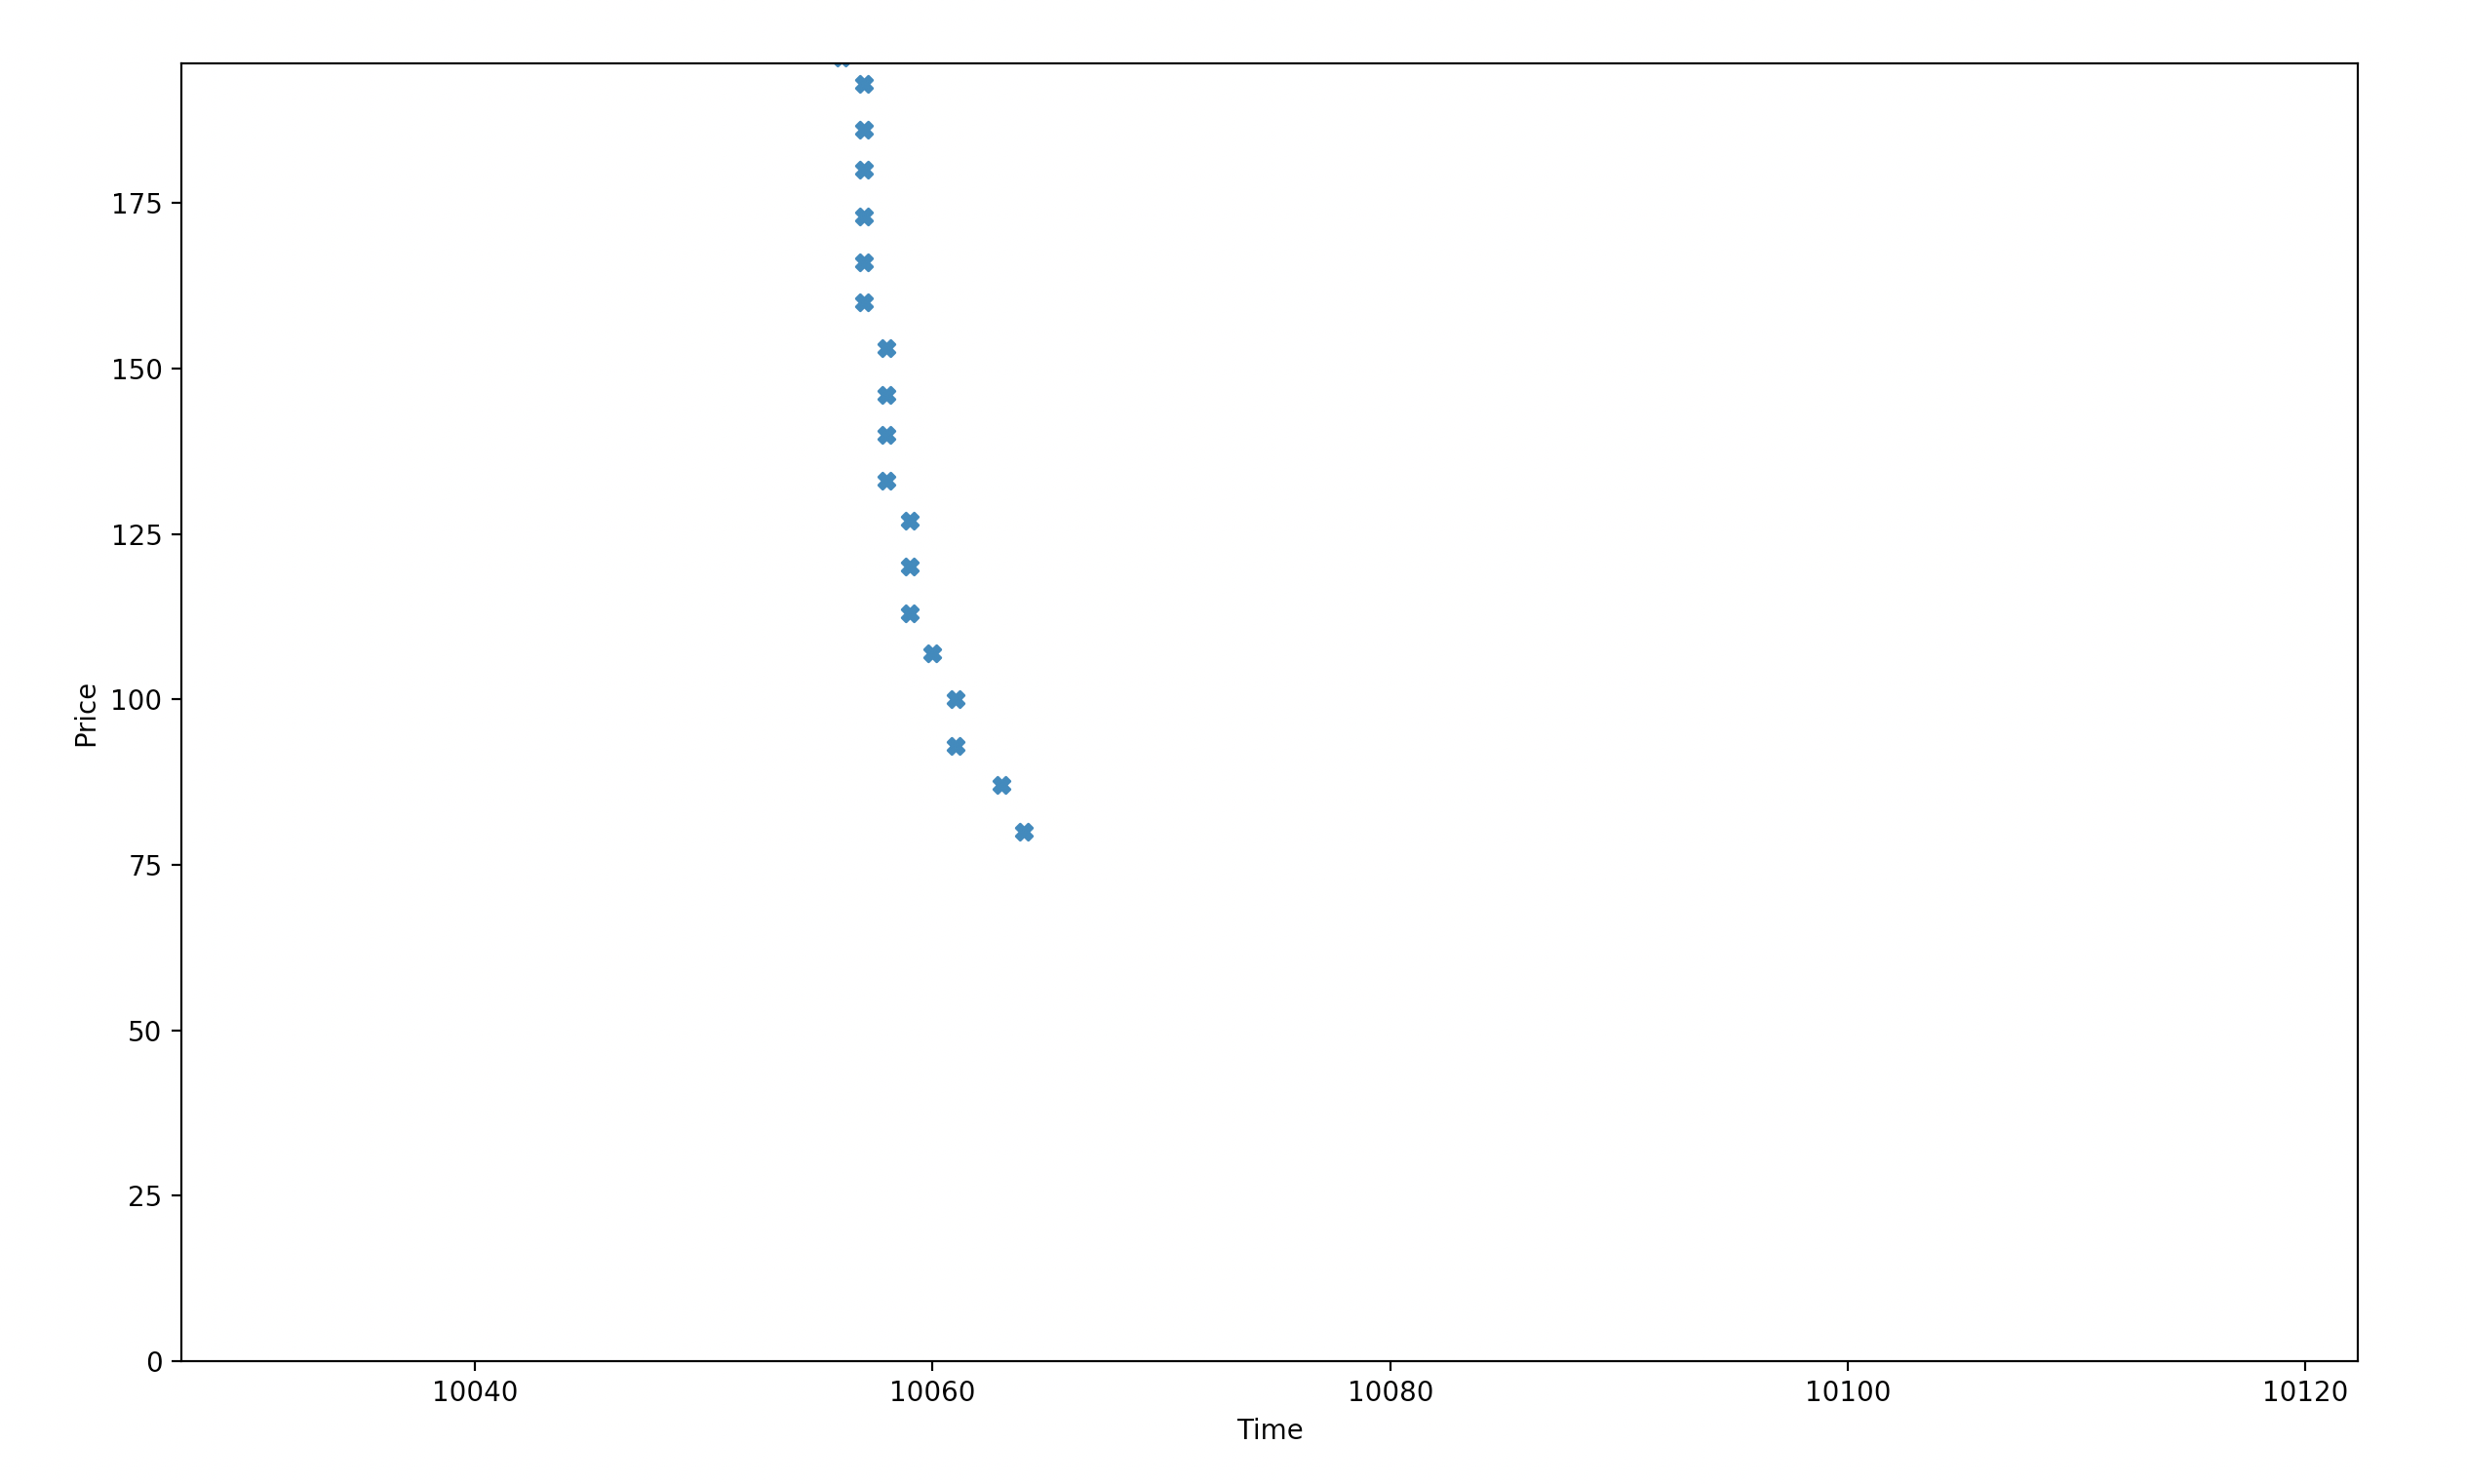
\includegraphics[ height=8cm]{Dissertation/images/snpr_adapted/zoom.png}
\caption{Zoomed-in graph of the Figure \ref{fig:SNIPER_FINAL}} 
\end{figure} 
\FloatBarrier

\subsection{ZI-C}
ZIC's behaviour in the new LOB is still similar to the one ran in the original BSE. The transaction price does not converge in any period of the session.

\begin{figure}[h]
\includegraphics[ height=8cm]{Dissertation/images/change2/zic.png}
\caption{62 ZI-C agents homogeneous market transaction diagram with 100 price equilibrium from McG action step implementation}  
\end{figure} 
\FloatBarrier

\subsection{ZI-P}
In ZIP's case, the implementation and adaptation is much more complex. In the experiment, the results suggest that the probability of acting for ZI-P agent (implemented so that it is similar to the McG agents) play a huge role in the convergence of ZI-P equilibrium. The parameter $p_{zip}$ is the probability of acting of the ZI-P agent. The adaptation is very similar to how McG adapted the Oesch's agents (Market maker and Liquidity consumer) to their model in which the Oesch's \cite{Oesch} time system is very similar to that of BSE's. The Figure \ref{fig:ZIP_prob_all} illustrate the examples of ZI-P converge in each probability. It can clearly be seen that as the probability decreases, the convergence will be better. In the 1 case, the ZI-P barely converges at all. However, as the probability in 0.5 and 0.25, the transaction price slowly converges near the equilibrium at 100. 

\begin{figure}[h]
  \begin{subfigure}[b]{0.5\textwidth}
    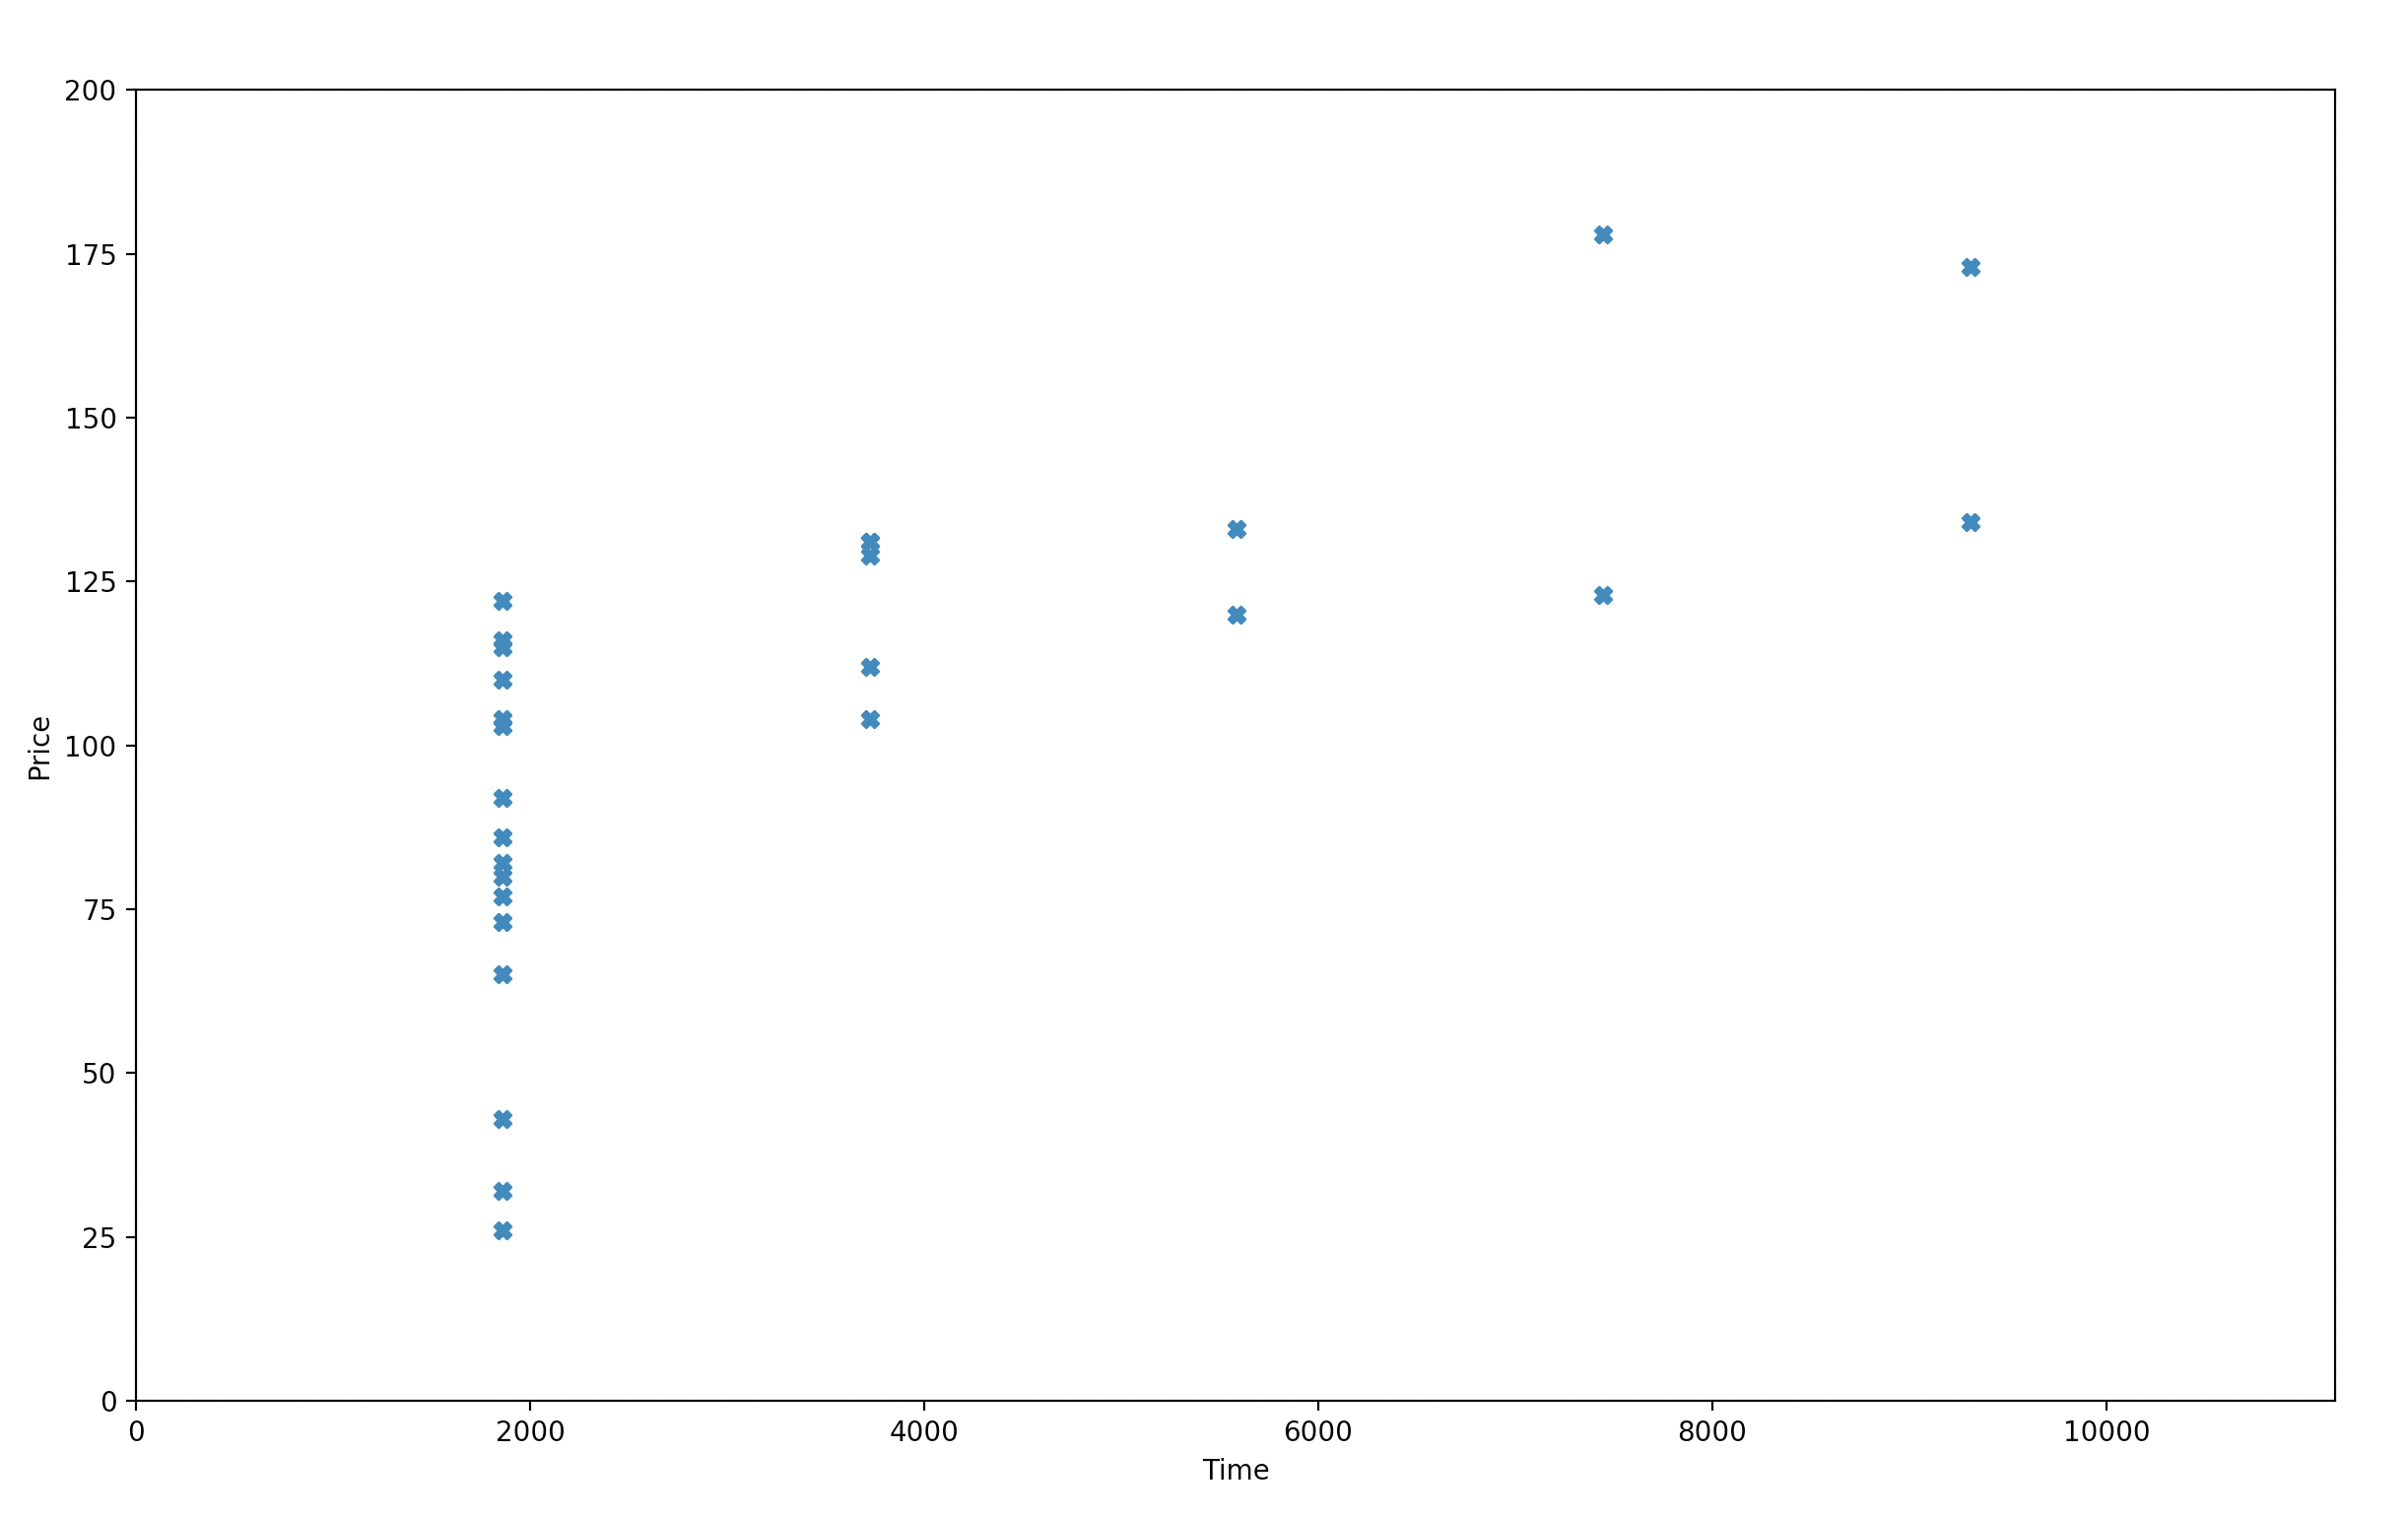
\includegraphics[width=7cm, height=7cm]{Dissertation/images/zip_randomized/1.png}
    \caption{ZI-P with $p_{zip} = 1$ }
    \label{fig:1}
  \end{subfigure}
  %
  \begin{subfigure}[b]{0.5\textwidth}
    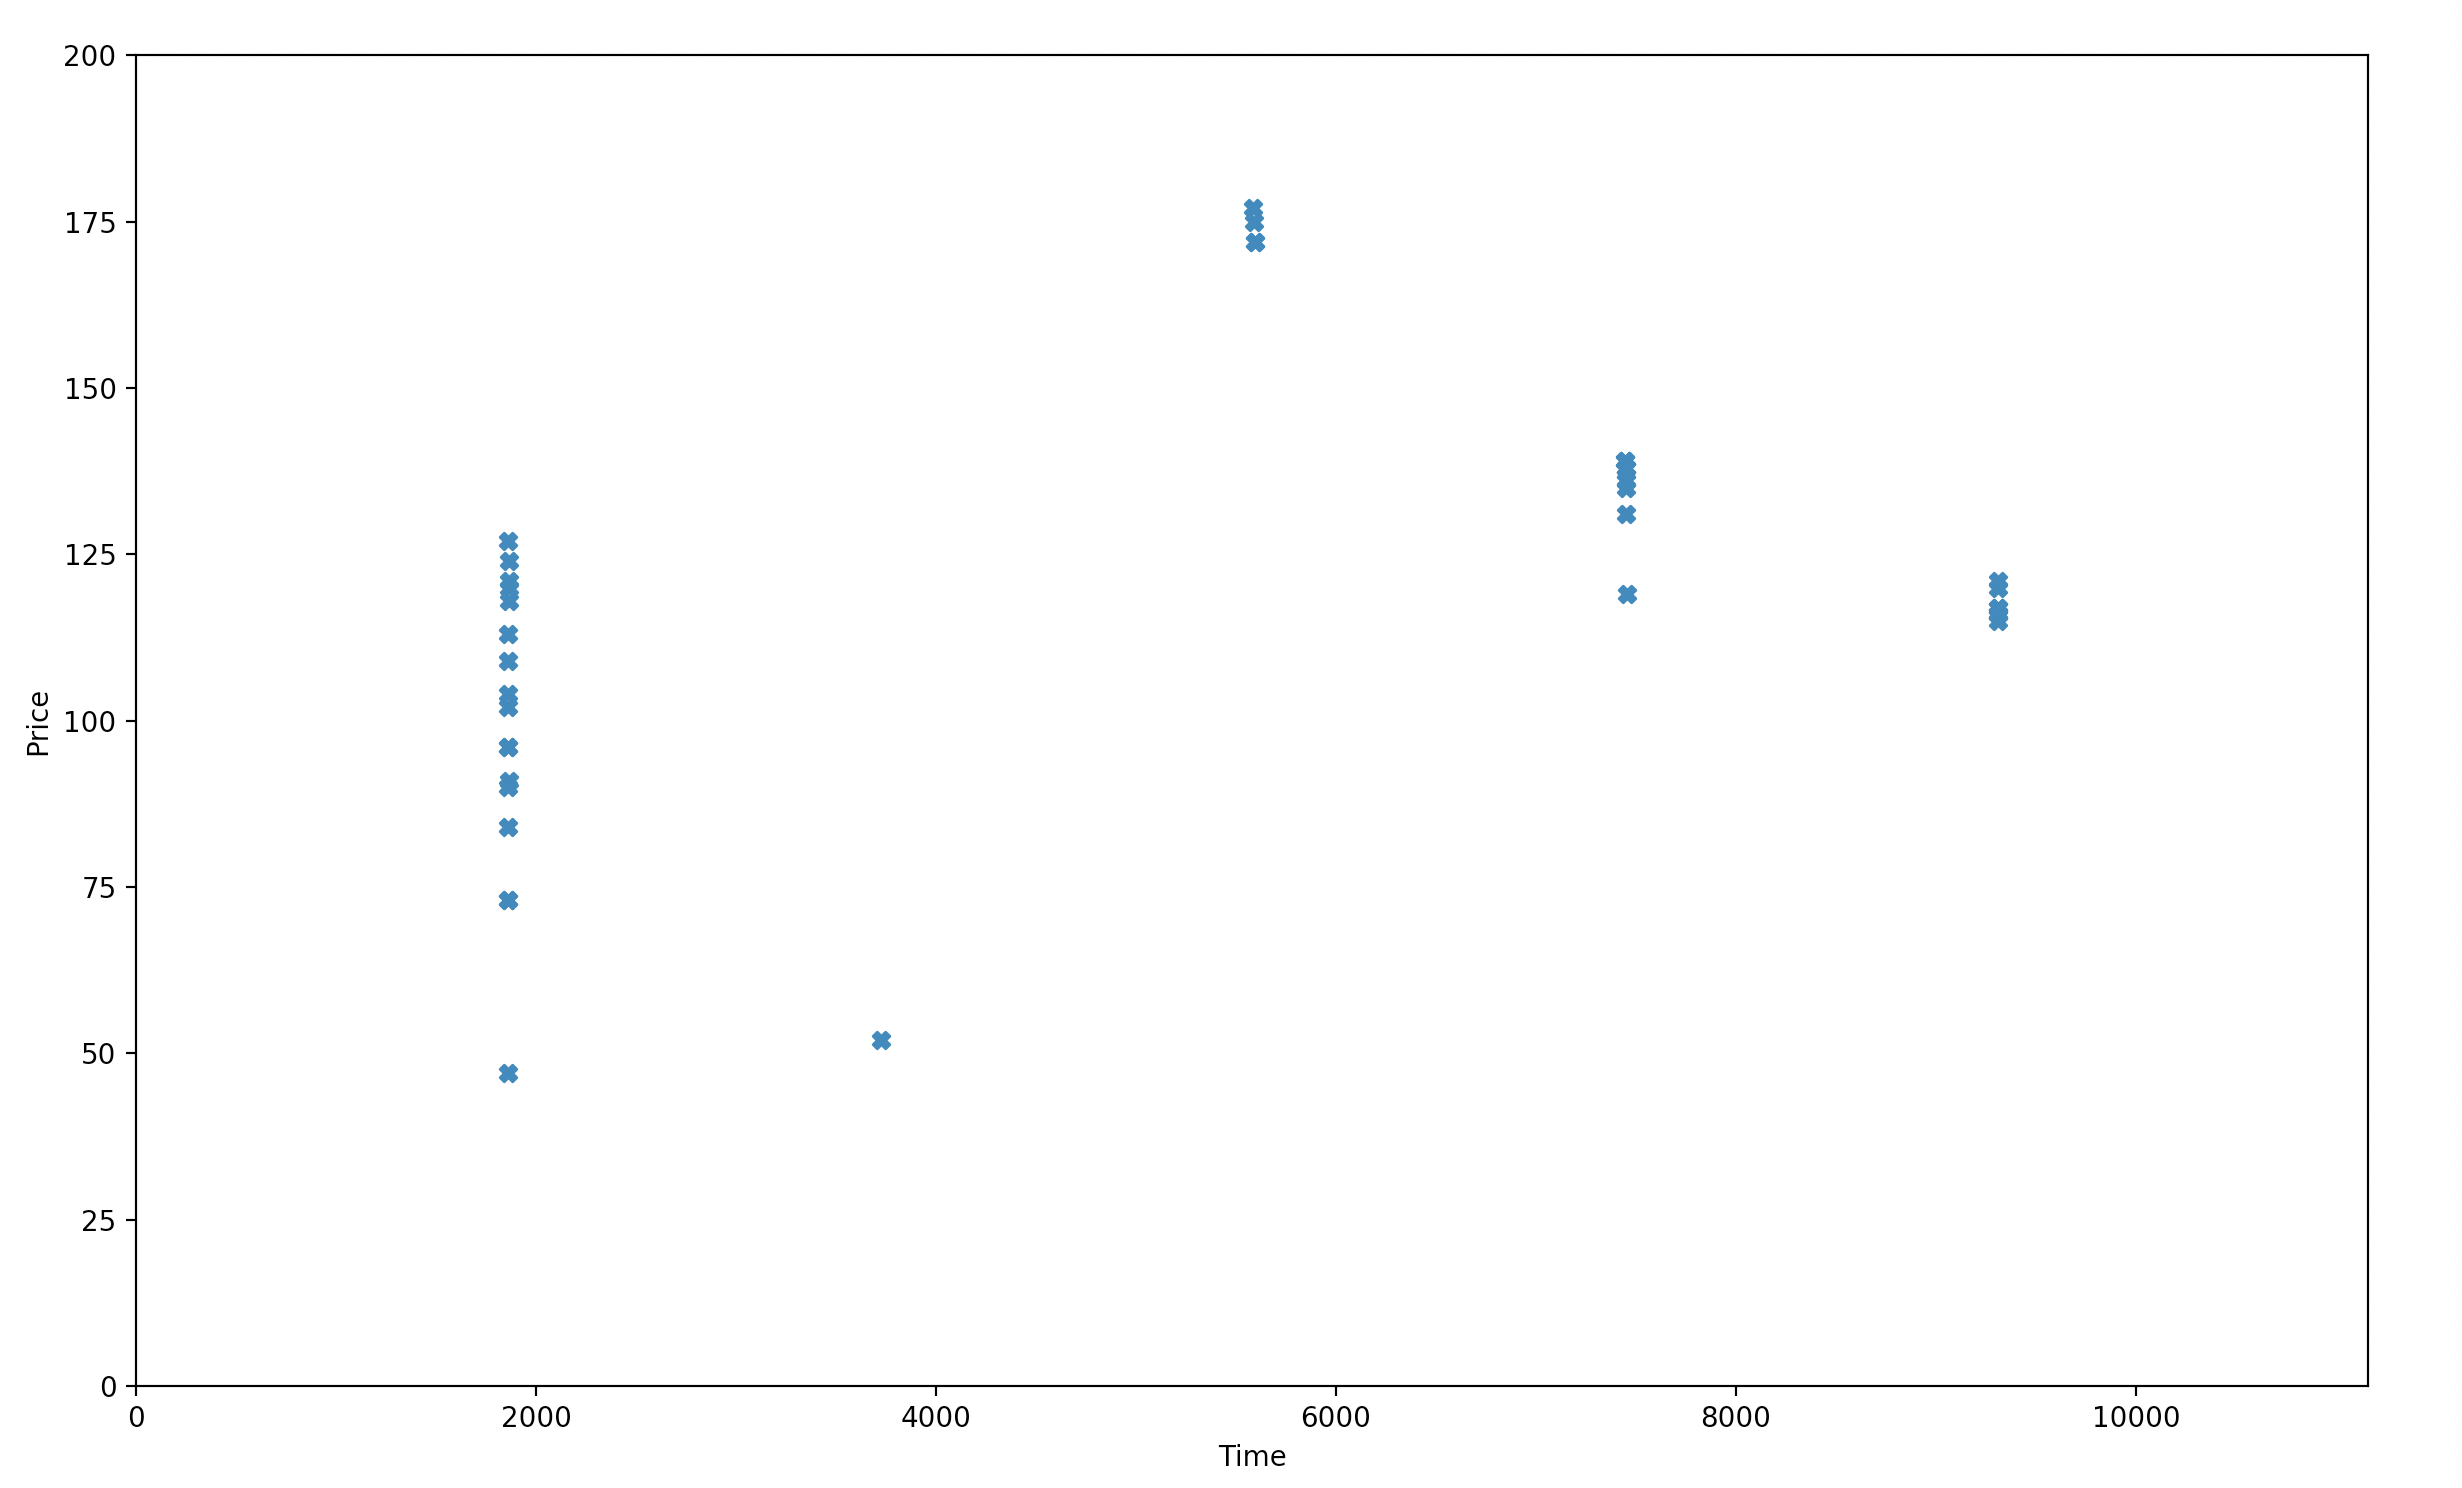
\includegraphics[width= 7cm, height=7cm]{Dissertation/images/zip_randomized/0.5.png}
    \caption{ZI-P with $p_{zip} = 0.5$}
    \label{fig:2}
  \end{subfigure}
\end{figure}

\begin{figure}[h]
  \begin{subfigure}[b]{0.5\textwidth}
    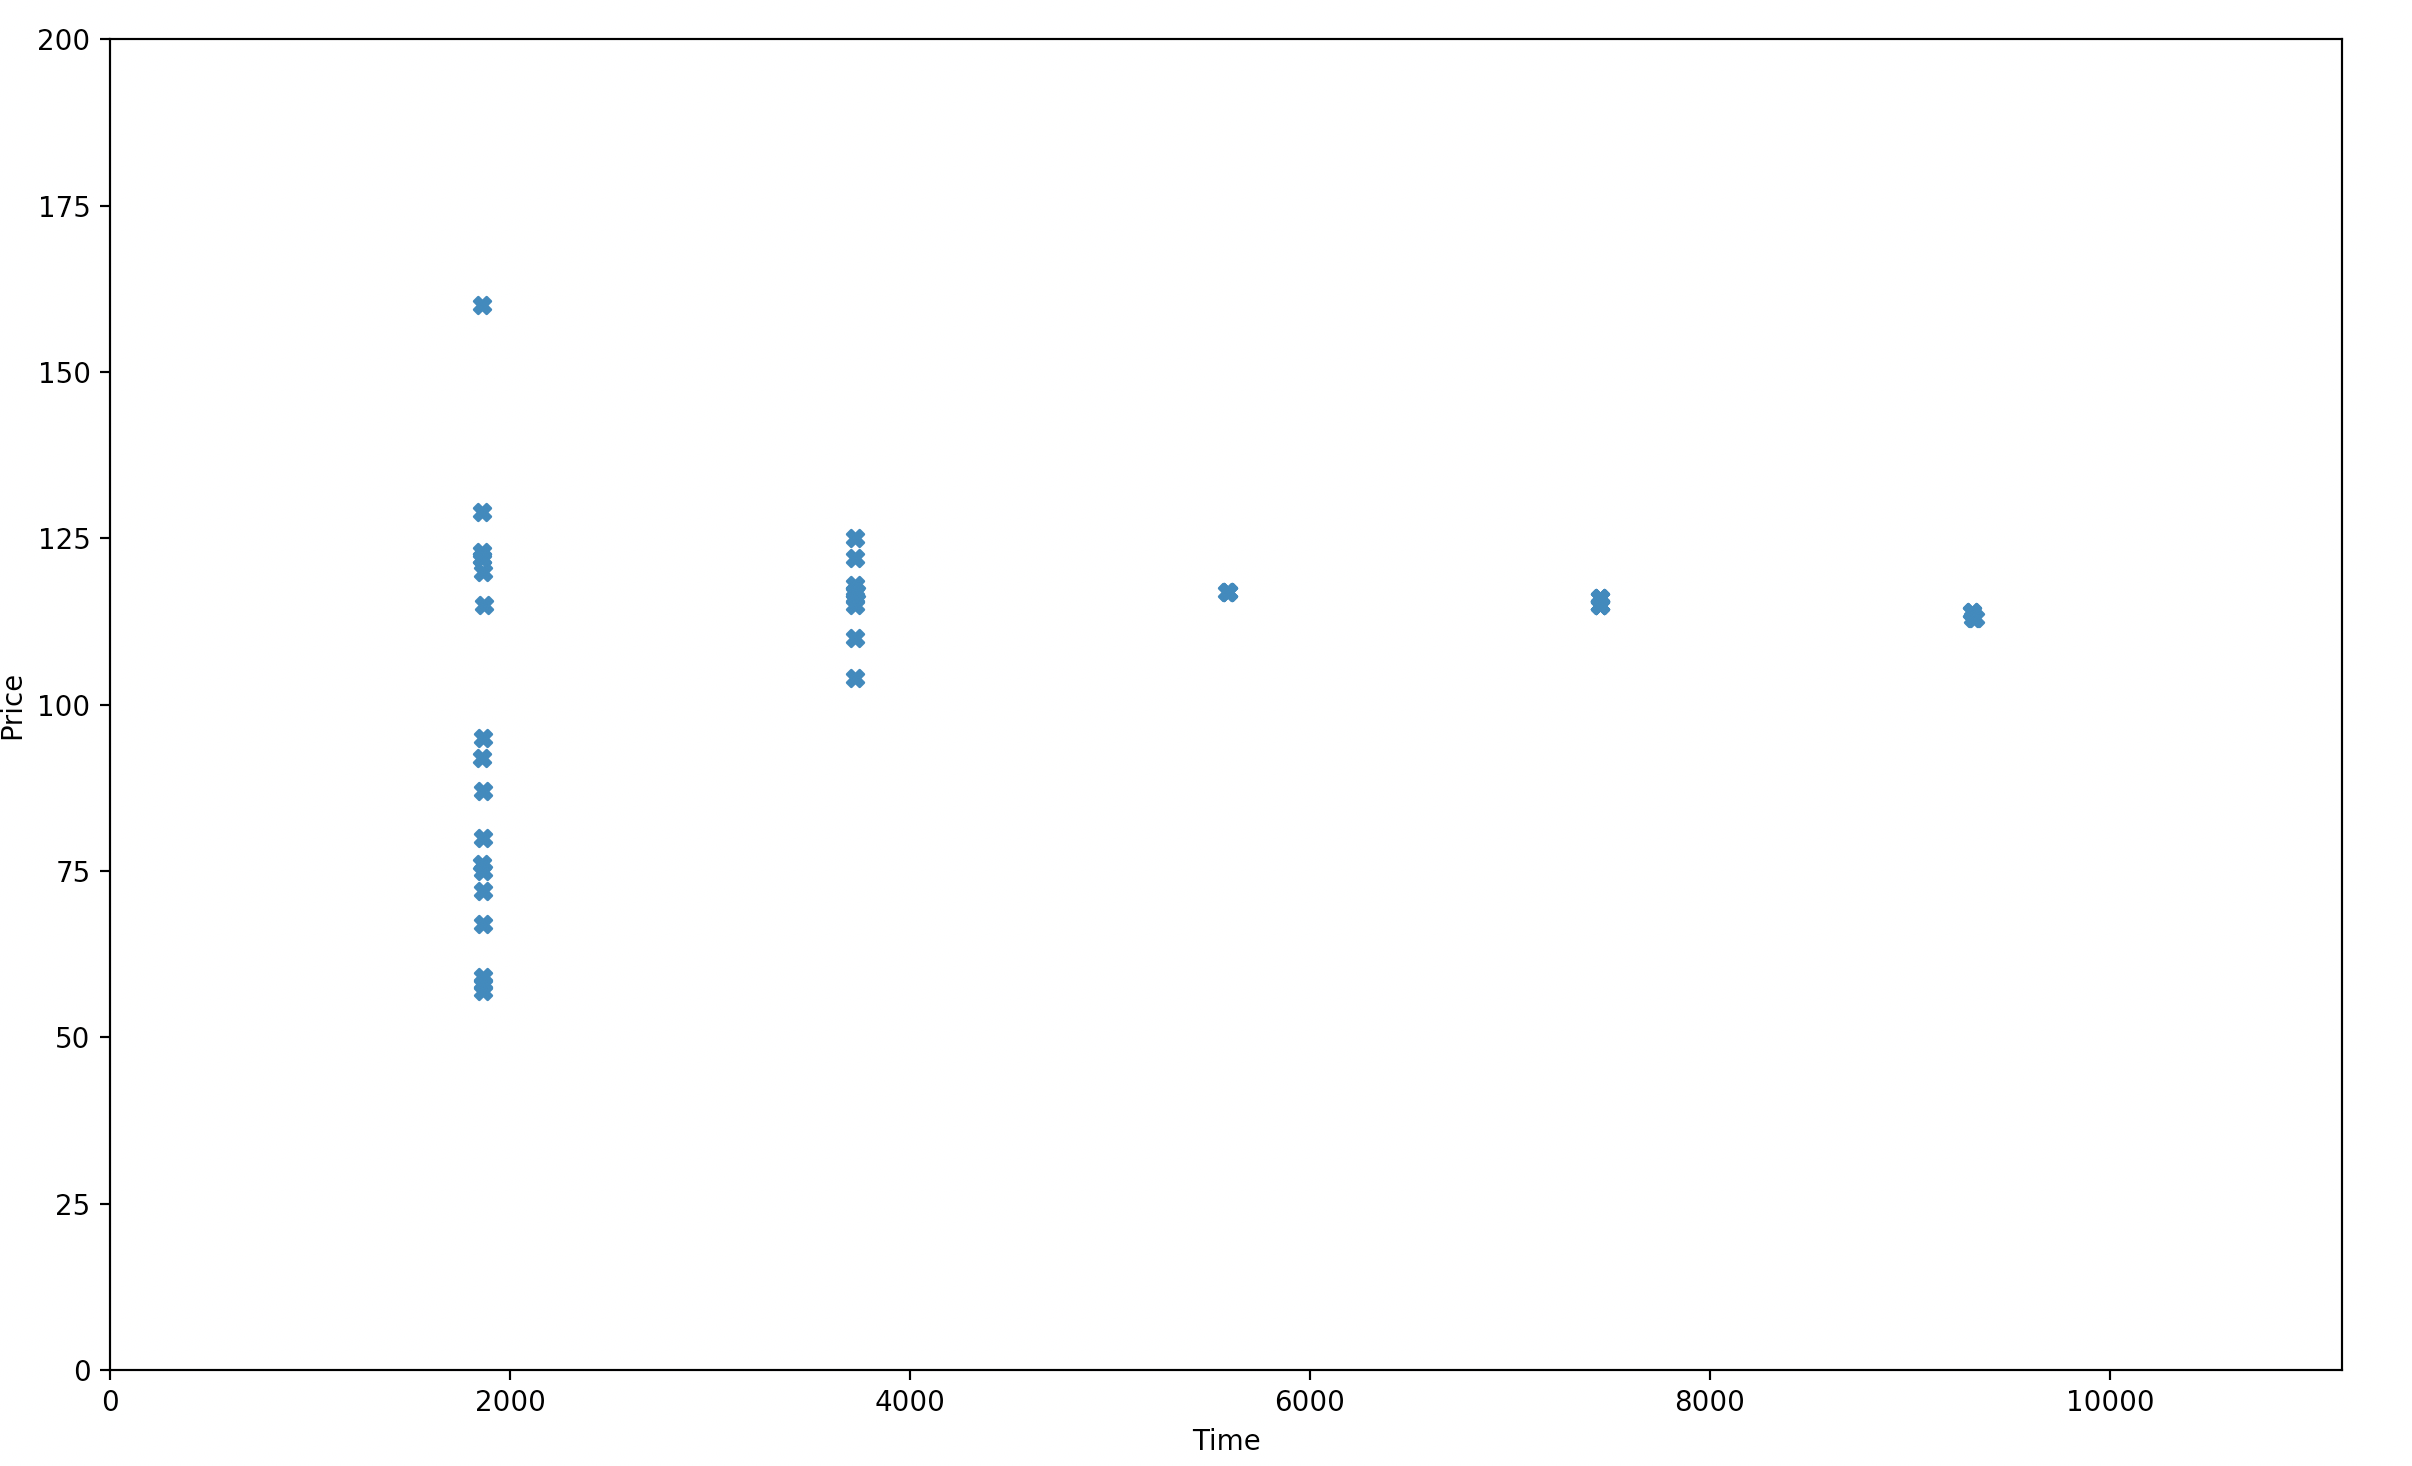
\includegraphics[width= 7cm, height=7cm]{Dissertation/images/zip_randomized/0.25.png}
    \caption{ZI-P with $p_{zip} = 0.25$}
    \label{fig:3}
  \end{subfigure}
  %
  \begin{subfigure}[b]{0.5\textwidth}
    \includegraphics[width= 7cm, height=7cm]{Dissertation/images/change2/zip.png}
    \caption{ZI-P with $p_{zip} = 0.1$}
    \label{fig:4}
  \end{subfigure}
\caption{Transaction diagrams of ZI-P with different probability of acting}
\label{fig:ZIP_prob_all}
\end{figure}

\begin{table}[h]
\centering
\begin{tabular}{ |m||p{4cm}|} 
\hline
\textbf{Probability}& \textbf{Smith's alpha value} \\
\hline
\hline
Original value & 24.8\\
\hline 
1 & 40.12 \\ 
\hline
0.5 & 41.12\\ 
\hline
0.25 & 32.0 \\ 
\hline
0.1 & 25.4 \\ 
\hline
\end{tabular}
\caption{Smith's alpha value after implementing probability of acting $p_{zip}$}  
\end{table}
\FloatBarrier
To illustrate this further, the figures below is the comparison between the final 0.1 probability with the original Base Line ZI-P behaviour. 

\begin{figure}[hbpt!]
  \begin{subfigure}[b]{0.5\textwidth}
    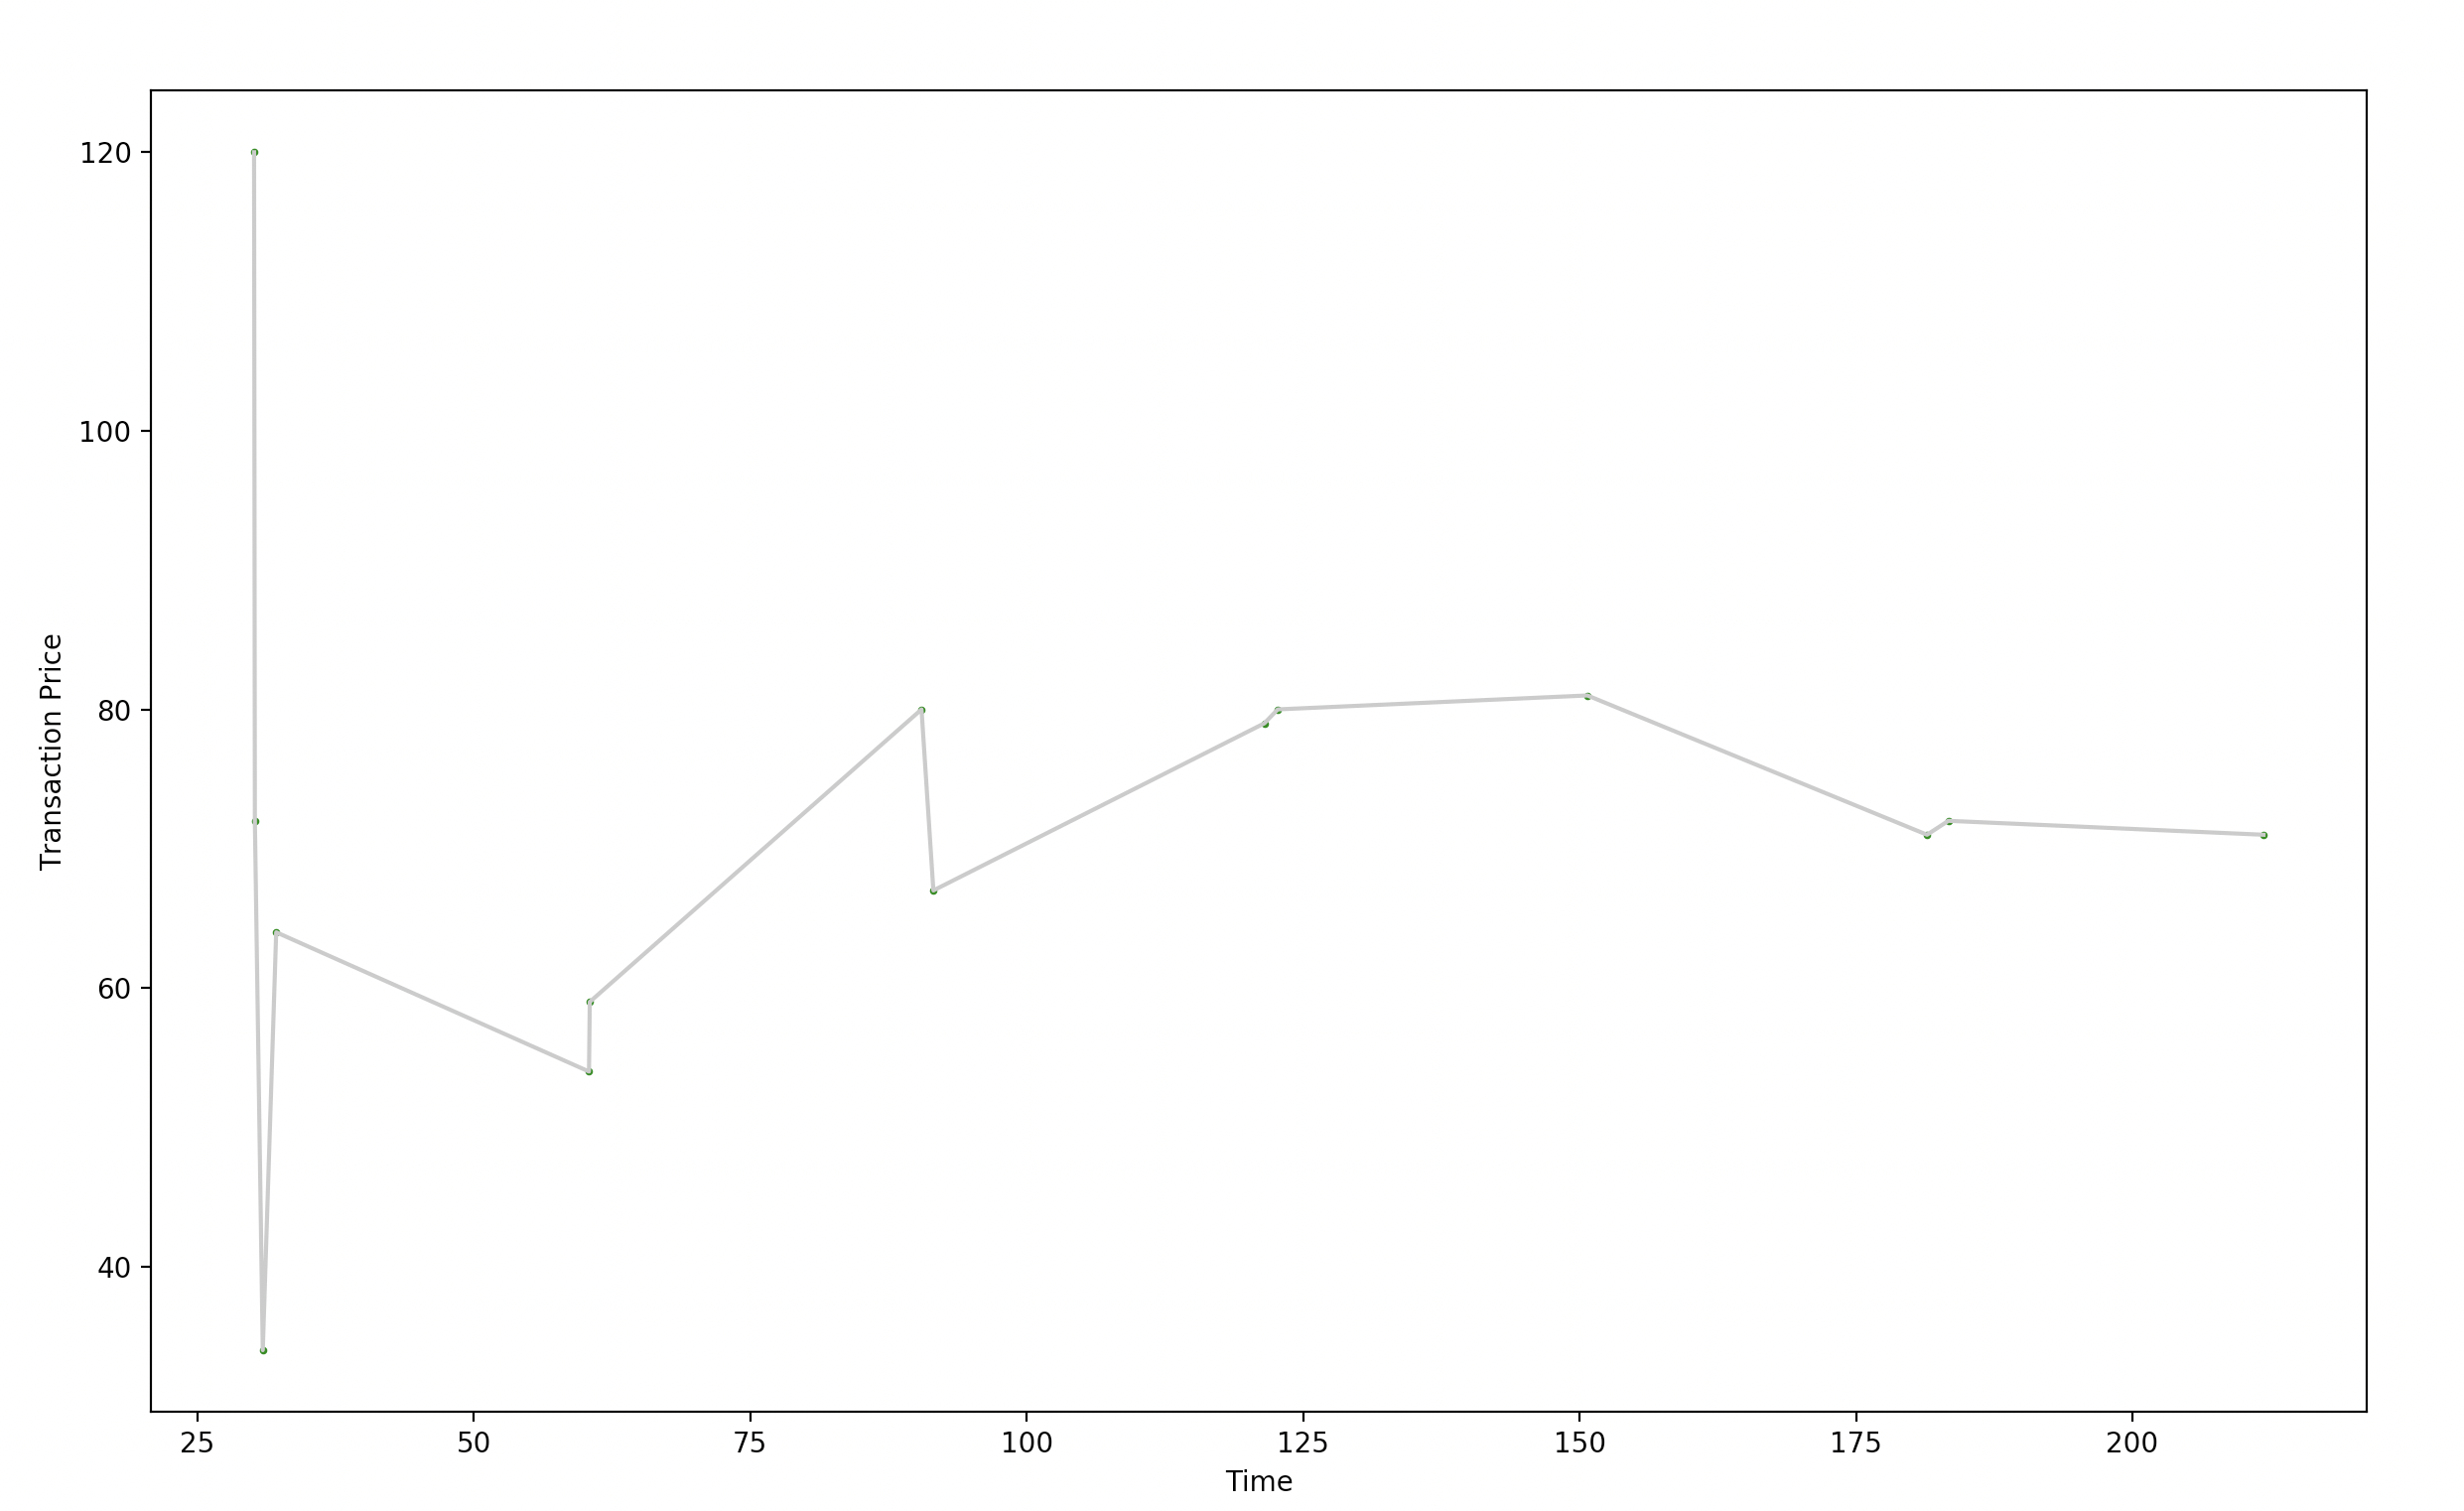
\includegraphics[ height=7cm, width = 7cm]{Dissertation/images/base_line/ZIP.png}
    \caption{Base Line ZI-P (same as Figure \ref{fig:ZIP_org_all}) }
    \label{fig:1}
  \end{subfigure}
  %
  \begin{subfigure}[b]{0.5\textwidth}
    \includegraphics[ height=7cm, width= 7cm]{Dissertation/images/change2/zip.png}
    \caption{ZI-P with $p_{zip} = 0.1$} 
    \label{fig:2}
  \end{subfigure}
\caption{Comparison of Base Line results of ZI-P and McG adapted parameter version} 
\end{figure}
\FloatBarrier

\section{Number of Transactions}
The table below illustrates the similarities of the number of transactions in each implementation of the BSE. As illustrated, the number of transactions in the market from the two new implementation versions are close to the original version of the BSE, hence is evidence that the agents are functioning properly. 

\begin{table}[h]
\centering
\begin{tabular}{ |m||p{4cm}|p{4cm}|p{4cm}|} 
\hline
\textbf{Agents}& \textbf{Base Line} & \textbf{Section 3.2 : Implemented Complex order types} & \textbf{Section 3.3: Implemented McG action step} \\
\hline
\hline
Kaplan's Sniper & 20 & 20 & 20 \\ 
\hline
ZI-C & 71 & 73 & 78\\ 
\hline
ZI-P & 42 & 45 & 47 \\ 
\hline
\end{tabular}
\caption{Number of transactions in each implementation}  
\end{table}
\FloatBarrier

\section{Evaluation}
This section's aim is to provide evidence that the market is function appropriately after implementing complex order types and McG action-steps. By evaluating the behaviours of the three existing agents : ZI-P, ZI-C and Sniper along with the Smith's alpha values, we can now established that the market is functional and stable. In the next chapter, we can now introduce new agents into the system. 